\def\ouexamdate{21 August 2006}
\def\ouexamversion{2.1.1}
\def\ouexamshortdate{2006/08/21}
% \iffalse meta-comment
%%%%%%%%%%%%%%%%%%%%%%%%%%%%%%%%%%%%%%%%%%%%%%%%%%%%%%%%%%%%%%%%%%%%%%%%%%%%%%%%
%%
%% File: $Id$
%% Copyright 1999--2006 Nigel Stanger and University of Otago
%% 
%% You may use this package freely, and also distribute it
%% provided that you don't change it, make any money off
%% it or pretend that you wrote it.
%%
%%%%%%%%%%%%%%%%%%%%%%%%%%%%%%%%%%%%%%%%%%%%%%%%%%%%%%%%%%%%%%%%%%%%%%%%%%%%%%%%
%<*driver>
\documentclass{ltxdoc}
\usepackage{doc}
\DisableCrossrefs
\CodelineNumbered
\RecordChanges

\usepackage{graphicx}
% change hyperref options as required
\usepackage[dvips,colorlinks,pdfpagemode=None,a4paper,urlcolor=blue,
            linkcolor=red,pdfauthor={Nigel Stanger}]{hyperref}

\title{The \textsf{ouexam} document class, v\ouexamversion}
\author{Nigel Stanger\\nstanger@infoscience.otago.ac.nz}
\date{\ouexamdate}

\begin{document}
\maketitle
\DocInput{ouexam.dtx}
\end{document}
%</driver>
%
% \fi
%
%% \CheckSum{807}
%%
%% \CharacterTable
%%  {Upper-case    \A\B\C\D\E\F\G\H\I\J\K\L\M\N\O\P\Q\R\S\T\U\V\W\X\Y\Z
%%   Lower-case    \a\b\c\d\e\f\g\h\i\j\k\l\m\n\o\p\q\r\s\t\u\v\w\x\y\z
%%   Digits        \0\1\2\3\4\5\6\7\8\9
%%   Exclamation   \!     Double quote  \"     Hash (number) \#
%%   Dollar        \$     Percent       \%     Ampersand     \&
%%   Acute accent  \'     Left paren    \(     Right paren   \)
%%   Asterisk      \*     Plus          \+     Comma         \,
%%   Minus         \-     Point         \.     Solidus       \/
%%   Colon         \:     Semicolon     \;     Less than     \<
%%   Equals        \=     Greater than  \>     Question mark \?
%%   Commercial at \@     Left bracket  \[     Backslash     \\
%%   Right bracket \]     Circumflex    \^     Underscore    \_
%%   Grave accent  \`     Left brace    \{     Vertical bar  \|
%%   Right brace   \}     Tilde         \~}
%%
%
% \MakeShortVerb{\|}
% 
% \changes{1.0}{1999/04/15}{Initial version.}
%
% \begin{abstract}
% This document class allows you to create Otago University final
% examination papers using \LaTeXe\@. It implements the major formatting
% requirements specified by the University, provides useful
% macros to ease the process of building the title page and automatically
% deals with fiddly little issues such as question and section numbering,
% the number of pages in the paper, printing ``\textbf{TURN OVER}'' in the
% bottom right corner of every page except the last one and ensuring that the
% total number of marks for a question adds up to the expected number.
% \end{abstract}
% 
% 
% \tableofcontents
% 
% 
% \section{Overview}
% 
% \changes{2.1}{2004/04/10}{NJS Added requirements and installation instructions.}
% \subsection{Requirements and installation}
% 
% The \textsf{ouexam} package requires only one other package: Rainer
% Sch\"{o}pf's \textsf{verbatim} package, which should come standard with
% most \TeX\ installations. To build the documentation and example files,
% you will need at least version 1.1 of the \textsf{listings} package, and
% GhostScript.
% 
% Installing is relatively simple:
% \begin{enumerate}
% 
% 	\item Unpack the distribution archive and \texttt{cd} to the
% 	distribution directory.
% 	
% 	\item \texttt{make}.
% 	
% 	\item \texttt{make install TEXMF\_INSTALL=/path/to/texmf}.
% 	\texttt{/path/to/texmf} should be the root of your preferred
% 	\texttt{texmf} tree (e.g., \texttt{/usr/share/texmf}). You may need
% 	to do this as root depending on which \texttt{texmf} tree you are
% 	installing into. You can also define \texttt{TEXMF\_INSTALL} as an
% 	environment variable then simply type \texttt{make install}.
% 
% \end{enumerate}
% You can, of course, always install manually if you wish.
% 
% 
% \changes{2.0}{2002/01/11}{NJS Added note on backwards compatibility.}
% \subsection{Important note on backwards compatibility}
% 
% Version 2.0 of \textsf{ouexam} introduces several major changes from earlier
% versions. Consequently, documents created using an earlier version of
% \textsf{ouexam} are \emph{incompatible} with version 2.0 or later. Versions 2.0
% and greater of \textsf{ouexam} will detect attempts to process version 1.x
% document and display an error message.
% 
% The older version (1.2) is still available and can be downloaded from the same
% location as the current version. To process older version documents, just copy
% the version 1.2 |ouexam.cls| file into the same directory as the document file.
% \TeX\ searches the current directory first, so this copy will take precedence
% over any other installed version of \textsf{ouexam}.
% 
% 
% \subsection{Class options}
%
% This document class is based on the \textsf{article} class and accepts any of
% the options accepted by \textsf{article}. The default options are
% \textsf{onecolumn}, \textsf{oneside}, \textsf{a4paper} and \textsf{12pt}.
% Normally the only one you might want to change is the last one.
% In addition, \textsf{ouexam} accepts the following ``native'' class options:
% \begin{description}
% 	\item[\textsf{draft}] \DescribeMacro{draft} This option has the usual
% 	effects that you would expect for \textsf{draft} mode in the
% 	\textsf{article} class, plus \fbox{DRAFT} is printed in
% 	the header of every page. Note that if you use the \textsf{graphicx}
% 	package and turn on the \textsf{draft} option in \textsf{ouexam}, all
% 	included graphics will be drawn in draft mode unless you specify the
% 	|draft=false| option to \cs{includegraphics}.
% 	
% 	\item[\textsf{markingschedule}] \DescribeMacro{markingschedule}
% 	Rather than write a separate marking schedule for an examination paper, you
% 	can use the \textsf{marking} environment to embed marking information
% 	within questions (see 
% 	\hyperref[Sec:Questions:Marking]{section~\ref*{Sec:Questions:Marking}}).
% 	By default this information is not printed (for obvious reasons!), but
% 	when it comes time to print a marking schedule for the examination,
% 	including the \textsf{markingschedule} class option in the
% 	\cs{usepackage} command will cause \textsf{ouexam} to print the hidden
% 	content. It will also print \fbox{MARKING SCHEDULE} in the footer of
% 	every page.
% \end{description}
% 
% 
% \subsection{Required packages}
% 
% This class requires the \textsf{verbatim} package in order to implement
% the marking schedule functionality.
% 
% 
% \subsection{Page margins}
% 
% This class assumes A4 paper. You will probably get weird results if you try
% to do anything different. The margins are set up as follows: top and bottom
% 2cm (headers and footers are inside this margin), left and right 2.54cm (1in).
% 
% 
% \changes{2.1.1}{2006/08/21}{NJS Updated \textsf{lastpage} style to display
% ``\textbf{END}''.}
% \subsection{Page styles}
% 
% There are three page styles defined in this class:
% \begin{description}
% 	\item[\textsf{plain}] \DescribeMacro{plain} This is a slight modification
% 	of the \textsf{plain} page style from \textsf{article}. It produces pages
% 	that have the page number centered at the top, the paper number in the top
% 	right corner and the text ``\textbf{TURN OVER}'' in the bottom right. This
% 	is the default page style.
% 	
% 	\item[\textsf{lastpage}] \DescribeMacro{lastpage} This is similar to
% 	\textsf{plain} but with ``\textbf{END}'' instead of ``\textbf{TURN
% 	OVER}''. It is used for the last page of the examination. You
% 	normally will not have to use this yourself---the class should take
% 	care of it automatically. The class does however occasionally seem
% 	to get confused, so there may times when you have to set the page
% 	style of the last page manually. It will be fairly obvious when you
% 	need to do this---the usual effect is that the last page
% 	has``\textbf{TURN OVER}'' printed on it when it should not.
% 	
% 	\item[\textsf{titlepage}] \DescribeMacro{titlepage} This is similar to
% 	\textsf{plain} but without the page header, and is used for the title page
% 	of the paper. As with \textsf{lastpage}, you will normally not use this
% 	yourself, because the \cs{maketitlepage} macro handles this automatically
% 	(see \hyperref[Sec:TitlePage]{section~\ref*{Sec:TitlePage}}).
% \end{description}
% 
% 
% \section{Writing an examination paper}
% 
% 
% \changes{2.0.2}{2002/05/11}{NJS Moved the title page subsection to the start
% of this section.}
% \subsection{The title page}
% \label{Sec:TitlePage}
% 
% This class defines a collection of macros that let you fill in the various
% parts of the examination title page. This is analogous to the process you use
% to generate the title of a document in, for example, the \textsf{article} class
% (using \cs{title}, \cs{author}, \cs{date} and \cs{maketitle}). That is, you
% issue the macros described below in the document preamble, then issue a
% \cs{maketitlepage} in the document body.
% 
% The \DescribeMacro{\examyear} \cs{examyear} macro lets you specify the year
% in which the examination is being held, for example, |\examyear{1999}|. This
% macro is mandatory.
% 
% The \DescribeMacro{\department} \cs{department} macro lets you specify the
% name of the department that produced the examination paper, for example,
% |\department{Information| |Science}|. This macro is mandatory.
% 
% The \DescribeMacro{\papernumber} \cs{papernumber} macro lets you specify the
% paper number that the examination is for, for example,
% |\papernumber{COMP 101}|. This macro is mandatory. \textbf{Warning:} Do not make
% the paper number string too long or it will overlap the page number. Be
% particularly careful when you specify semester information using \cs{semester},
% because this is appended to the paper number in the page header. For example,
% if you specify |\papernumber{COMP 101}| and |\semester{2}|, the header will
% contain ``COMP 101 (Semester Two)'' rather than just ``COMP 101''. The worst
% case you will need to consider in such situations is a special examination,
% which inserts the text ``(Special Examination)'' after the paper number.
% 
% The \DescribeMacro{\papertitle} \cs{papertitle} macro lets you specify the
% title of the paper, for example, 
% |\papertitle{Systems Analysis and Design Methods}|. This macro is mandatory.
% 
% \changes{2.0.2}{2002/08/22}{NJS Added `FY' to the \cs{semester} macro
% description.}
% Some papers are offered in more than one semester. The
% \DescribeMacro{\semester} \cs{semester} macro lets you specify which
% semester the examination is for. The argument can be either ``1'' or ``2''
% for semesters 1 and 2, ``SS'' for summer school, ``FY'' for a full-year
% paper or ``SP'' for a special examination, for example, |\semester{2}|.
% Invalid values for the argument cause a warning to be raised. This macro is
% optional---if you omit it, no semester information is generated.
% 
% The \DescribeMacro{\timeallowed} \cs{timeallowed} macro lets you specify the
% length of the examination in hours, for example, |\timeallowed{2}|. This
% macro is optional---if you omit it, it defaults to three (3) hours.
% 
% \changes{2.1}{2004/04/05}{NJS Modified \cs{allowcalculators} to conform
% to the new University calculator regulations.}
% \changes{2.1}{2004/04/05}{NJS Added \cs{permitcalculators} as a synonym
% for \cs{allowcalculators}.}
% If calculators are permitted in the examination, use the
% \DescribeMacro{\allowcalculators}
% \DescribeMacro{\permitcalculators}
% \cs{allowcalculators} macro (\cs{permitcalculators} will also work).
% This macro is optional---if you omit it, a sentence is inserted saying
% that calculators are \emph{not} permitted. \cs{allowcalculators} has a
% single optional argument that specifies the kind of calculators
% permitted. If omitted, it defaults to ``any'' (see below). Otherwise,
% this argument must be one of the following values:
% \begin{description}
% 
% 	\item[none:] a sentence is inserted noting that no calculators are
% 	permitted.
% 
% 	\item[approved:] a sentence is inserted noting that only approved
% 	calculators are permitted.
% 
% 	\item[any (default):] a sentence is inserted noting that any
% 	calculator that does not have a communication capability is
% 	permitted.
% 
% \end{description}
% 
% The \DescribeMacro{\instructions} \cs{instructions} macro lets you specify
% instructions on how candidates should complete the
% examination, for example, |\instructions{Answer ALL| |questions.}|. This macro
% is optional. Note that the content of the instructions can be just about
% anything. It is up to you to control formatting, such as how you want lines
% broken, etc. This also true of the \cs{material}, \cs{copiesof} and
% \cs{otherinstructions} macros described below.
% 
% The \DescribeMacro{\material} \cs{material} macro lets you specify any
% additional material that candidates are provided in addition to the
% examination paper itself, for example, |\material{SQL schema definition}|.
% This macro is optional.
% 
% The \DescribeMacro{\copiesof} \cs{copiesof} macro lets you specify any
% material that candidates are allowed to bring into the examination, for
% example, |\copiesof{McFadden &| |Hoffer, 5th edition}|. This macro is
% optional.
% 
% The \DescribeMacro{\otherinstructions} \cs{otherinstructions} macro lets you
% specify any other instructions not covered by any of the above, for example,
% |\otherinstructions{No smoking| |allowed.}|. This macro is optional.
% 
% Once you have specified the content of the title page using the above
% macros, you simply issue a \DescribeMacro{\maketitlepage} \cs{maketitlepage}
% to generate the front page of the examination (cf. \cs{maketitle}). The title
% page generated meets University formatting requirements.
% Note that the number of pages in the examination paper is generated
% and inserted into the title page automatically---you do not need to specify
% it manually.
% 
% 
% \subsection{Sections}
% \label{Sec:Sections}
% 
% Examination papers may optionally have multiple sections, ``numbered'' A,
% B, \ldots. Rather than redefine the existing section macros, this class
% defines an \DescribeEnv{examsection} \textsf{examsection}
% environment\footnote{Note that the old \cs{newsection} macro has been
% retained for backwards compatibility with earlier development versions of
% \textsf{ouexam}. The \textsf{examsection} environment replaces this macro
% and should be used in all new documents.} that generates a new section. The
% \textsf{examsection} environment has three mandatory arguments:
% \begin{enumerate}
% 	\item The expected number of marks for the question. If you leave this
% 	argument empty it defaults to zero. \textsf{ouexam} keeps a running total
% 	of the \emph{actual} number of marks encountered within a section, which is
% 	compared with the value of this argument when the environment is closed.
% 	An error is raised if the values are not equal. The running total is also
% 	typeset right-justified in the form ``\textbf{[SECTION A TOTAL 20 MARKS]}''
% 	as an additional verification.
% 	
% 	\item Instructions for answering questions in this section (such as
% 	``Answer any TWO questions.''). If you leave this argument empty it
% 	defaults to ``ANSWER ALL QUESTIONS.''.
% 	
% 	\item A description of the topic of the section. This can be left
% 	empty.
% \end{enumerate}
% Every section begins on a new page, and the section title is formatted as
% ``\textbf{\underline{Section A}}'', in \cs{large} size. For example:	\\
% 
% \noindent|\begin{examsection}{25}{}{These questions are remarkably boring.}|	\\
% \hspace*{1cm}\vdots	\\
% |\end{examsection}|	\\
% 
% \noindent will produce the following (assuming that the actual number of
% marks in the question is correct):
% 
% \begin{center}
% 	\fbox{%
% 	\begin{minipage}{0.9\columnwidth}
% 		{\large\noindent\textbf{\underline{Section~A}}}	\\[0.5\baselineskip]
% 		ANSWER ALL QUESTIONS.	\\
% 		These questions are remarkably boring.	\\
% 		\hspace*{2cm}\vdots	\\
% 		\mbox{}\hfill\textbf{[SECTION A TOTAL 25 MARKS]}
% 	\end{minipage}
% 	}
% \end{center}
% 
% 
% \subsection{Questions}
% \label{Sec:Questions}
% 
% \textsf{ouexam} provides three environments for building examination
% questions: \DescribeEnv{question} \textsf{question},
% \DescribeEnv{subquestion} \textsf{subquestion} and \textsf{subsubquestion},
% which correspond to top-level questions, parts of questions, and
% \DescribeEnv{subsubquestion} sub-parts of questions respectively. They
% produce questions that are numbered according to University examination
% formatting requirements. Note that questions are normally numbered
% sequentially throughout the entire paper regardless of any section
% boundaries.
% 
% All three environments have a single mandatory argument which is the
% expected number of marks for the question, part or sub-part. If this
% argument is left empty it will default to zero. This argument works in much
% the same way as the first argument to the \textsf{examsection} environment
% (see \hyperref[Sec:Sections]{section~\ref*{Sec:Sections}}): \textsf{ouexam}
% keeps a running total of the number of marks encountered within each
% question part and sub-part, and compares this total with the expected value
% when the environment closes. Where appropriate, the running total is
% typeset right-justified in the form ``(5 marks)''. For example:
% \begin{verbatim}
% \begin{question}{5}
%   \begin{subquestion}{2}
%     Why is the sky blue?
%   \end{subquestion}
%   \begin{subquestion}{3}
%     Explain in detail how the sky can be made pink.
%   \end{subquestion}
% \end{question}
% \begin{question}{1}
%   Define the term ``floccinaucinihilipilification''.
% \end{question}
% \end{verbatim}
% 
% \noindent will produce the following:
% \begin{center}
% 	\fbox{%
% 	\begin{minipage}{0.9\columnwidth}
% 		\begin{enumerate}
% 			\item
% 			\begin{enumerate}
% 				\item Why is the sky blue? \hfill (2 marks)
% 
% 				\item Explain in detail how the sky can be made pink. \hfill (3
% 				marks)
% 			\end{enumerate}
% 
% 			\item Define the term ``floccinaucinihilipilification''. \hfill (1
% 			mark)
% 		\end{enumerate}
% 	\end{minipage}
% 	}
% \end{center}
% 
% The \textsf{question} environments handle formatting of marks totals
% automatically, including considerations such as:
% \begin{itemize}
% 	\item whether or not to print the number of marks for a question at all
% 	(they should not be printed if the question has sub-parts);
% 	
% 	\item whether to print ``mark'' or ``marks'' (e.g., question 2 above); and
% 	
% 	\item where to position the number of marks relative to the question,
% 	depending on how full the last line of the question is.
% \end{itemize}
%
% 
% \subsection{Marking schedule information}
% \label{Sec:Questions:Marking}
% 
% Rather than writing a separate marking schedule for an examination paper,
% you can use the \DescribeEnv{marking} \textsf{marking} environment to embed
% marking information within questions. By default this information is not
% printed (for obvious reasons!), but when it comes time to print a marking
% schedule for the examination, use the \textsf{markingschedule} class option
% to print the hidden content. The marking information will be printed in
% \emph{italics} to differentiate it from the main body of the examination,
% and \fbox{MARKING SCHEDULE} will also be printed in the footer of every
% page.
% 
% \changes{2.1}{2004/04/10}{NJS Added driver file tip.}
% A useful tip for writing examination papers is to create two separate
% ``driver'' documents that are set up the document class for the
% ``plain'' and ``marking schedule'' versions of the examination,
% respectively. Each should then include a separate document that contains
% the actual content of the examination paper, for example:
% 
% \begin{verbatim}
% \documentclass[markingschedule]{ouexam}
% 
% \input{exampaper} % contains the actual examination content
% \end{verbatim}
% 
% Doing this enables you to build the ``plain'' and ``marking schedule''
% versions independently, without overwriting each other or having to
% change the original source file. Simply run \LaTeX\ on the appropriate
% driver file to produce the version that you want. See the example files
% that came with the \textsf{ouexam} distribution for an example of this
% approach in action.
% 
% 
% \subsection{Miscellaneous}
% 
% Most examinationss are marked out of 100, and \textsf{ouexam} defaults to
% this. However, if you want an examination that is marked out of some other
% number, for example, 90 marks, you can specify this using the
% \DescribeMacro{\examoutof} \cs{examoutof} macro. Thus, |\examoutof{90}|
% will set the expected number of marks for the examination to 90. This value
% is used by \textsf{ouexam} to verify that the marks for all the questions
% add up to the expected number of marks for the examination.
% 
% 
% \section{Errors and warnings}
% 
% In this section are described the error messages and warning produced by
% \textsf{ouexam}, and the reasons why they occur.
% 
% 
% \subsection{Error messages}
% 
% \noindent\texttt{INCOMPATIBLE (\ldots): this document was written for an
% earlier}	\\
% \texttt{version of ouexam \ldots}	\\
% You are trying to use v2.0 or later of \textsf{ouexam} with a document that
% was written for \textsf{ouexam} v1.2 or earlier. Versions 2.0 and later of
% \textsf{ouexam} are \emph{fundamentally incompatible} with earlier
% versions. The only solutions here are either to revert to \textsf{ouexam}
% v1.2 or earlier (you can put a copy of the class file in the same directory
% as the document), or rewrite the document to conform to the current version
% of \textsf{ouexam}. You should be able to download a copy of v1.2 from the
% same location that you found the current version.	\\
% 	
% \noindent\texttt{no \cs{examyear} was specified}	\\
% \noindent\texttt{no \cs{department} was specified}	\\
% \noindent\texttt{no \cs{papernumber} was specified}	\\
% \noindent\texttt{no \cs{papertitle} was specified}	\\
% You have not specified one of these macros. All four of these macros are
% mandatory and must be included in the preamble of any \textsf{ouexam}
% document.	\\
% 
% 
% \subsection{Warnings}
% 
% \noindent\texttt{actual number of marks for exam (\ldots) does not match
% expected}	\\
% \texttt{number of marks (\ldots)}	\\
% The actual number of marks supplied for the whole examination (calculated
% by summing the marks for all the questions) is not the same as the expected
% total for the examination. Adjust the marks for the questions until the
% totals match.	\\
% 
% \noindent\texttt{actual mark (\ldots) for section \ldots\ does not match
% expected}	\\
% \texttt{mark (\ldots)}	\\
% The actual number of marks supplied for a particular section (calculated by
% summing the marks for all the questions in that section) is not the same as
% the expected total for that section. Adjust the marks for the questions in
% the section concerned until the totals match. The section number is given
% in the warning.	\\
% 
% \noindent\texttt{actual mark (\ldots) for question \ldots\ does not match
% expected}	\\
% \texttt{mark (\ldots)}	\\
% The actual number of marks supplied for a particular question (calculated
% by summing the marks of all its sub-parts) is not the same as the expected
% total for that question. Adjust the marks for the sub-parts of the
% question until the totals match. The question number is given
% in the warning.	\\
% 
% \noindent\texttt{DEPRECATED: The \cs{newsection} macro is deprecated; use
% the}	\\
% \texttt{examsection environment instead}	\\
% The \cs{newsection} macro is a hangover from earlier versions of
% \textsf{ouexam}, and has been left in v2.0 for backwards compatibility with
% some documents that use it. The entire sectioning mechanism was rewritten
% from scratch for v2.0, so this macro is now deprecated and will eventually
% disappear. You should use the \textsf{examsection} environment
% instead.	\\
% 
% \changes{2.0.2}{2002/08/22}{NJS Added `FY' to \cs{semester} error
% description.}
% \noindent\texttt{invalid value `\ldots' for \cs{semester}; valid values are
% `1', `2', `SS',}	\\*
% \texttt{`FY' and `SP'. No semester information will be printed}	\\*
% You have given an invalid value as the argument to the \cs{semester}
% macro. The allowed values are ``1'' (semester one), ``2'' (semester
% two), ``SS'' (summer school), ``FY'' (full-year) and ``SP'' (special
% examination). Any other values will be ignored. Note that these are
% case-sensitive, for example, `sp' is invalid. 	\\
% 
% \changes{2.1}{2004/04/05}{NJS Added \cs{allowcalculators} error
% description.}
% \noindent\texttt{invalid value `\ldots' for \cs{allowcalculators}; valid values are	\\*
% `none', `any' and `approved'. No calculators will be permitted}	\\*
% You have given an invalid value as the argument to the
% \cs{allowcalculators} macro. The allowed values are ``none'' (no
% calculators permitted), ``any'' (any calculator permitted) and
% ``approved'' (only approved calculators permitted). Any other values
% will be ignored, and \textsf{ouexam} will assume that no calculators are
% permitted. Note that these are case-sensitive, for example, `NONE' is
% invalid. 	\\
% 
% 
% \section{Example}
% 
% \changes{2.1}{2004/04/10}{NJS Updated example to conform to 2.1 changes.}
% \changes{2.0}{2002/01/25}{NJS Updated example to conform to 2.0 changes.}
% \changes{1.1}{1999/04/20}{NJS Updated example to conform to 1.1 changes.}
% The code given below is for the first three pages of the INFO~321 2001
% final examination. The output produced by this source is shown in
% \hyperref[Fig.Example]{figure~\ref*{Fig.Example} on
% page~\pageref*{Fig.Example}}. Particular points to note in this example
% are:
% \begin{itemize}
% 
% 	\item The number of hours is not specified, so it defaults to three.
% 
% 	\item This examination allows only approved calculators.
% 	
% 	\item The \textsf{listings} package (v1.1 or later) is used to
% 	typeset code listings.
% 
% 	\item The argument of the \cs{instructions} macro can be just about
% 	anything, as can the arguments of the \cs{material}, \cs{copiesof} and
% 	\cs{otherinstructions} macros. In this example, the \cs{instructions}
% 	macro has been omitted, causing \textsf{ouexam} to output the default
%	instructions.
% 
% 	\item Marking schedule information has been embedded within the
% 	questions. \hyperref[Fig.Example2]{Figure~\ref*{Fig.Example2} on
% 	page~\pageref*{Fig.Example2}} shows the output produced by this source
% 	when the \textsf{markingschedule} class option is used.
% 
% \end{itemize}
% The full source for this example may be found in the
% \texttt{example*.tex} files that came with this distribution.
% 
% \small
% \begin{verbatim}
% \documentclass{ouexam}
% 
% \usepackage{graphicx}
% \usepackage{listings}
% 
% \examyear{2001}
% \department{Information Science}
% \papernumber{INFO 321}
% \papertitle{Database Systems}
% \allowcalculators[approved]
% 
% \begin{document}
% 
% \lstloadlanguages{ODL,OQL,[Oracle8]SQL,[Oracle8]PLSQL}
% \lstset{basicstyle=\sffamily, showstringspaces=false, tabsize=2,
%   xleftmargin=1cm, belowskip=0pt, commentstyle=\itshape,
%   numbers=left, numberstyle=\scriptsize, numbersep=5pt,
%   columns=fullflexible,}
% 
% \maketitlepage
% 
% \begin{examsection}{25}{}{Questions in this section (total 25 marks) 
%   relate to physical database design and tuning.}
% 
% 
% 
% \begin{question}{10}
% 
%   A major U.S. mail order firm is having performance problems with queries
%   on the \textsf{Customer} table in its Oracle8 order-processing database.
%   Consider the following information about the \textsf{Customer} table,
%   then answer the questions below:	\\
% 
%   \textsf{\textbf{Customer}(\underline{customer\_no}, name, address, city,
%   state, country, phone, email, status)}
% 
%   \begin{itemize}
%     \item \textsf{customer\_no} is the primary key and because this is an
%     Oracle8 database, a unique B-tree index has been automatically created
%     on this column.
% 
%     \item \textsf{status} is a single character column that holds one of
%     the values `I' (inactive), `B' (bronze), `S' (silver) or `G' (gold).
%     The value of this column is determined by a customer's order history.
% 
%     \item About 10\% of customers are inactive, about 50\% have bronze
%     status, about 35\% have silver status and about 5\% have gold status.
% 
%     \item The average row size is about 200 bytes and there are
%     approximately 5,000,000 rows.
% 
%     \item The \textsf{Customer} table is heavily queried (averaging thirty
%     new queries per minute) by four different groups of employees. Group~1
%     queries only inactive customers, group~2 queries only bronze status
%     customers and groups~3 and~4 both query only silver and gold status
%     customers. Members of any group may query the table at any time and
%     queries often overlap.
% 
%     \item UPDATE, INSERT and DELETE operations on the table are uncommon.
% 
%     \item Very few queries are for individual customers; rather, most
%     queries are based on various combinations of values from
%     \textsf{status}, \textsf{city}, \textsf{state} and \textsf{country}.
%   \end{itemize}\medskip
% 
%   \begin{subquestion}{3}
%     Describe and justify an \emph{index-based} physical tuning solution
%     that will improve the performance of queries on the \textsf{Customer}
%     table. (No code is required.)
%     \begin{marking}
%       Since queries tend to be on combinations of several low-cardinality
%       columns [1] and the table is very large [1], the most effective
%       solution would be to place bitmap indexes on status, city, state and
%       country [1].
% 
%       B-tree indexes on any of the individual columns would not be ideal
%       because of their low cardinality. A possible alternative is a
%       composite B-tree index on all four columns [1 for suggesting this if
%       appropriate], but this is not ideal and would be much larger than
%       the four bitmap indexes [1 for this explanation if appropriate].
%       Hashing is definitely \emph{not} an option, because very few queries
%       are exact match.
%     \end{marking}
%   \end{subquestion}
% 
%   \begin{subquestion}{7}
%     \begin{subsubquestion}{5}\label{nonindex}
%       Assuming that there are two identical fast disks available, describe
%       and justify two alternative \emph{non index-based} physical tuning
%       solutions that will improve the performance of queries on the
%       \textsf{Customer} table. For each solution include details of how
%       the two disks will be used. (No code is required.)
%       \begin{marking}
%         Alternative 1: partition the table across the two disks based on
%         status (four partitions, one for each status value) [1]. This will
%         allow simultaneous parallel access to different parts of the table
%         by the different groups [1]. Since two groups both access silver
%         and gold customers, it makes sense to put the silver customers on
%         disk one and the gold customers on disk two. Bronze customers
%         account for 50\% of the table, so it makes sense to also put them
%         on disk two (as the gold customers are the smallest group), and
%         put the inactive customers on disk one with the silver customers.
%         [1 for any sensible partitioning scheme]
%   
%         Alternative 2: replicate the table across both disks (one replica
%         on each disk) [1]. This will also provide simultaneous parallel
%         access to the data (hard to tell whether this would be better or
%         worse than the partitioning above) [1].
%   
%         Note that any solution must be capable of being implemented in
%         Oracle8.
%       \end{marking}
%     \end{subsubquestion}
% 
%     \begin{subsubquestion}{2}
%       Briefly discuss the relative advantages and/or disadvantages of the
%       two alternative solutions you described in part~(\ref{nonindex})
%       above.
%       \begin{marking}
%         The partitioning solution given above doesn't really help with the
%         bronze customer rows---we would need random horizontal
%         partitioning to really help with this, which Oracle8 doesn't
%         support. More generally, Oracle8 does not migrate rows into the
%         correct partition if a customer's status changes, so the data will
%         need to be reloaded occasionally [1].
% 
%         For replication, we have the usual problem of keeping the replicas
%         synchronised if they are both read/write. This is somewhat
%         mitigated by the fact that there are only two copies [1].
%       \end{marking}
%     \end{subsubquestion}
%   \end{subquestion}
% \end{question}
% 
% \newpage
% \begin{question}{10}
%   There are two generic parameters that affect the structure of a B-tree
%   index.
% 
%   \begin{subquestion}{6}
%     Identify these two parameters and describe what each parameter
%     specifies. Use diagrams to illustrate your answer.
%     \begin{marking}
%       \emph{Node size} [1] specifies the maximum number of pointers in
%       each index node [1]. Suitable diagram [1].
% 
%       \emph{Percentage fill} [1] specifies the number of pointers in each
%       index node that are allocated when a node is created [1]. In effect,
%       it determines the amount of free space left in each node. Suitable
%       diagram [1].
%     \end{marking}
%   \end{subquestion}
%   
%   \begin{subquestion}{4}
%     For each of the two parameters, discuss the practical effect(s) of:
%     \begin{subsubquestion}{2}
%       high values of the parameter; and
%       \begin{marking}
%         Large node size reduces the height of the B-tree, resulting in
%         potentially fewer I/Os to access a leaf node [$\frac{1}{2}$]. It
%         can however increase the number of rows locked in a single leaf
%         node [$\frac{1}{2}$].
%   
%         High percent fill means that most pointers in a node will be
%         allocated when the node is created [$\frac{1}{2}$]. This leaves
%         little free space in the B-tree for new key values or key values
%         that change [$\frac{1}{2}$].
%       \end{marking}
%     \end{subsubquestion}
%     \begin{subsubquestion}{2}
%       low values of the parameter.
%       \begin{marking}
%         Small node size increases the height of the B-tree, resulting in
%         potentially more I/Os to access a leaf node [$\frac{1}{2}$]. The
%         number of rows locked in a single leaf node will be reduced
%         [$\frac{1}{2}$].
%   
%         Low percent fill means that most pointers in a node will not be
%         allocated when the node is created [$\frac{1}{2}$]. This leaves
%         little free space in the B-tree for new key values or key values
%         that change [$\frac{1}{2}$].
%       \end{marking}
%     \end{subsubquestion}
%   \end{subquestion}
% \end{question}
%   
%   
%   
% \begin{question}{5}\label{clusterq}
% 
%   \begin{subquestion}{2}
%     Define what is meant by the term ``clustering'' in the context of
%     physical database design and tuning, and explain why it is beneficial.
% 
%     \begin{marking}
%       Clustering is the grouping of related rows physically near to each
%       other on disk [1] so that they may be retrieved in as few I/Os as
%       possible (ideally one)---beneficial because of the slowness of disk
%       I/O compared to memory I/O [1].
%     \end{marking}
%   \end{subquestion}
%   
%   \begin{subquestion}{3}\label{clusterqcode}
%     Consider the following Oracle8 SQL table definition:
%     
%     \begin{lstlisting}[language={[Oracle8]SQL}]{}
% create table enrolment
% (  student_id char(7),
%   paper_code char(7),
%   enrol_year number(4),
%   
%   primary key (student_id, paper_code, enrol_year)
% );
%     \end{lstlisting}
% 
%     The \textsf{Enrolment} table is often queried for all rows relating to
%     a particular student in a particular year (for example, student
%     1234567 in 1998, student 9876543 in 2000, etc.). Write appropriate
%     Oracle8 SQL code that will cluster the rows of the table in such a way
%     as to support these types of query (you do not need to calculate
%     cluster sizes). Relevant Oracle8 syntax diagrams are given on the next
%     page.
%     \begin{marking}
%       \begin{lstlisting}[language={[Oracle8]SQL}]{}
% create cluster enrolment_cluster (student_id char(7), year number(4));
% 
% create index enrol_cluster_index on cluster enrolment_cluster;
% 
% create table enrolment
% (  student_id char(7),
%   paper_code char(7),
%   enrol_year number(4),
%   
%   primary key (student_id, paper_code, enrol_year)
% ) cluster enrolment_cluster(student_id, enrol_year);
%       \end{lstlisting}
%     \end{marking}
%     [1] each for correct cluster, cluster index and table clustering.
%   \end{subquestion}
% 
% \end{question}
% 
% \end{examsection}
%       .
%       .
%       .
% \end{document}
% \end{verbatim}
% \normalsize
% 
% \begin{figure}
% 	\fbox{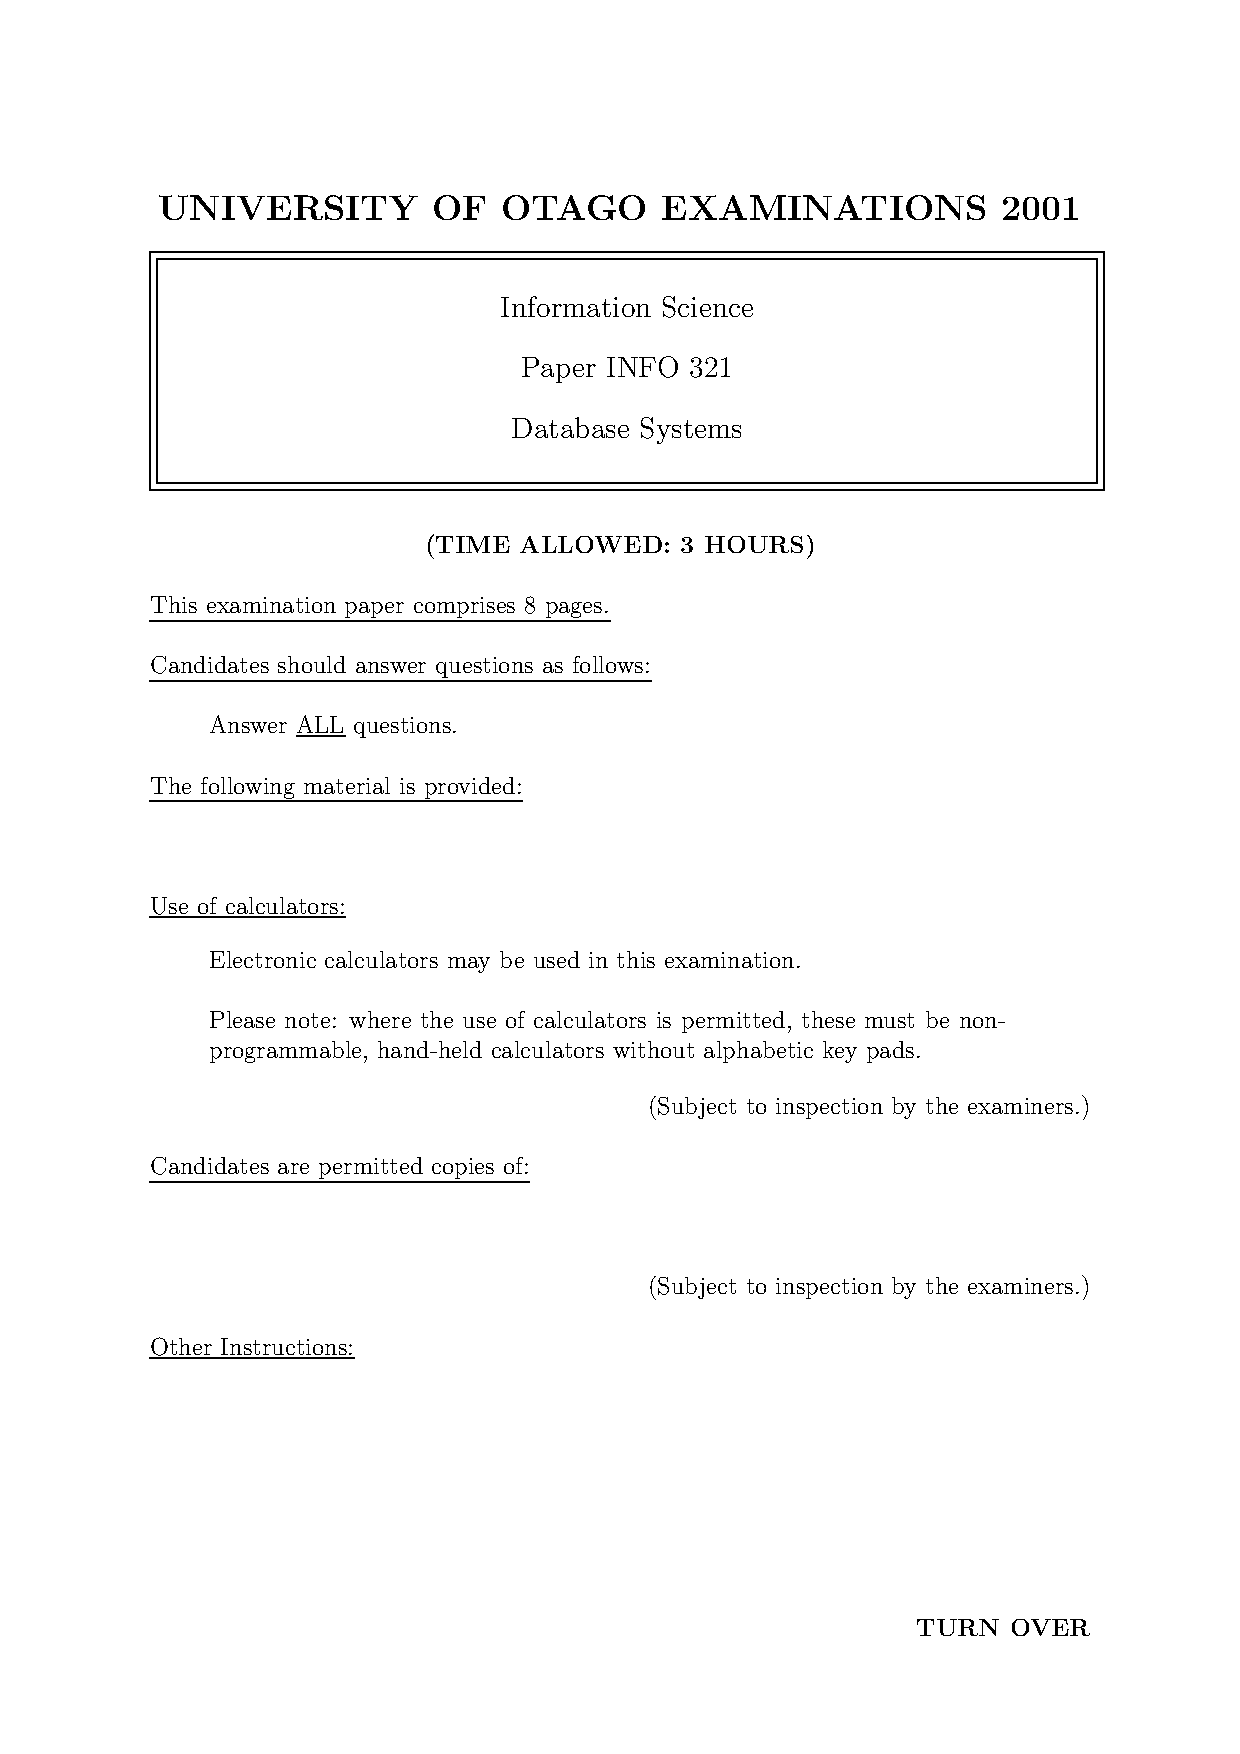
\includegraphics[bb=0 -57 596 785,scale=0.28]{eg1-1}}
% 	\hfill
% 	\fbox{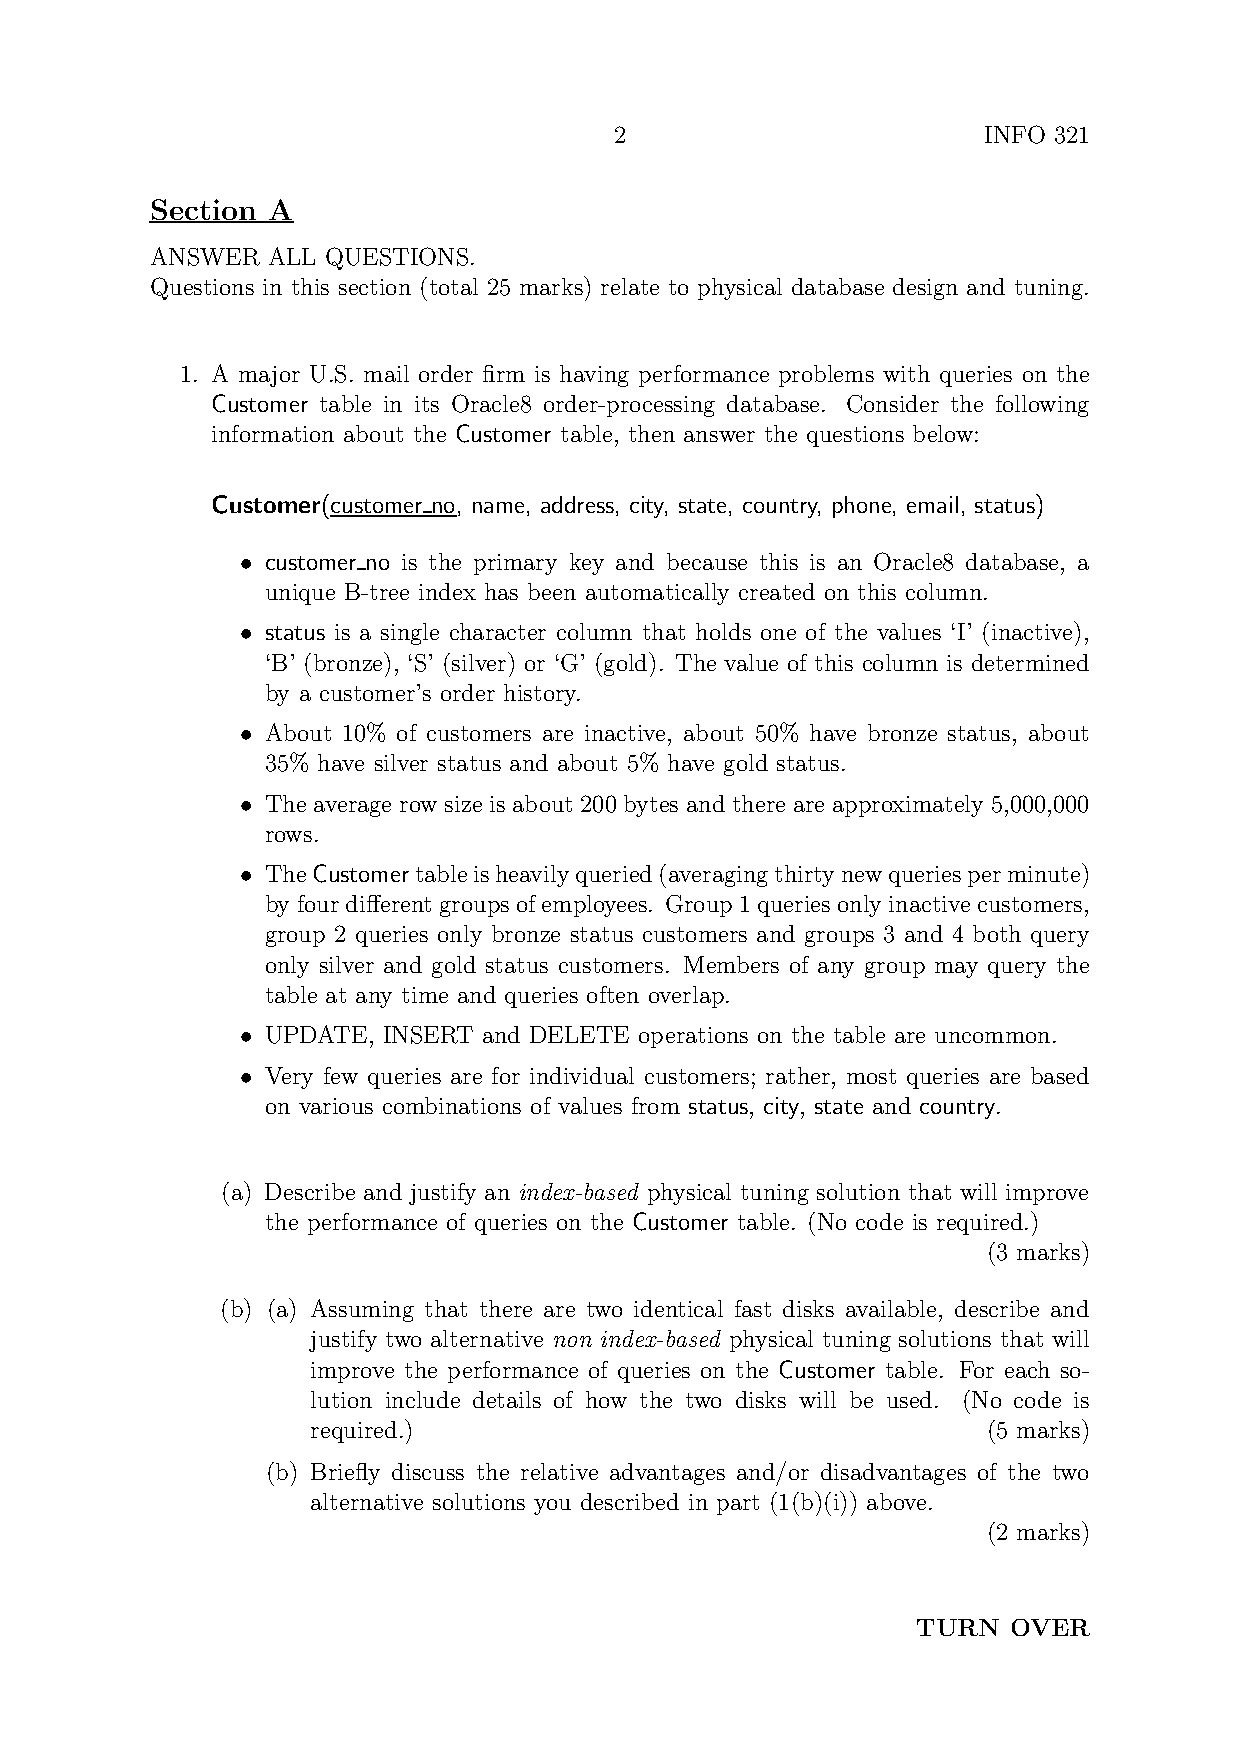
\includegraphics[bb=0 -57 596 785,scale=0.28]{eg1-2}}
% 	
% 	\begin{center}
% 		\fbox{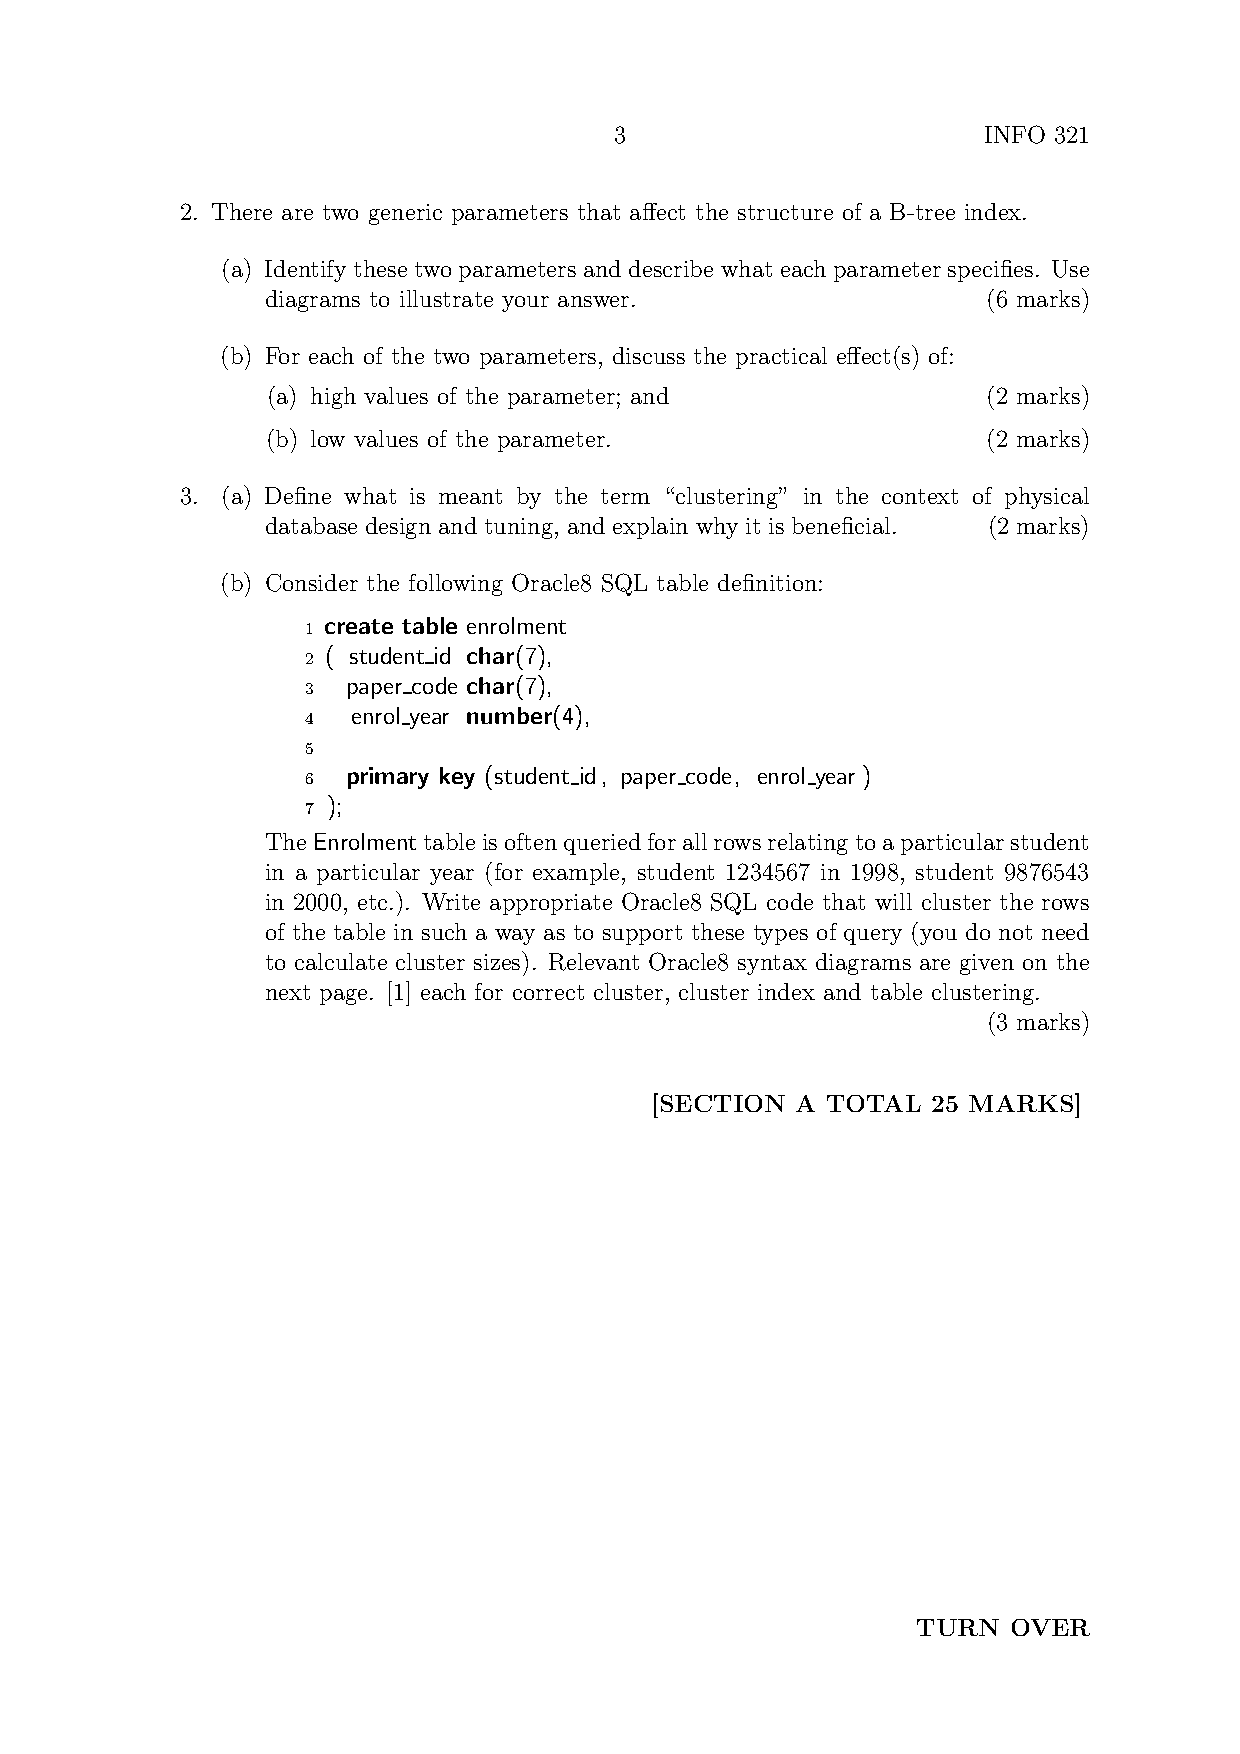
\includegraphics[bb=0 -57 596 785,scale=0.28]{eg1-3}}
% 	\end{center}
% 
% 	\caption{Output produced by \textsf{ouexam}.}
% 	\label{Fig.Example}
% \end{figure}
% 
% \begin{figure}
% 	\fbox{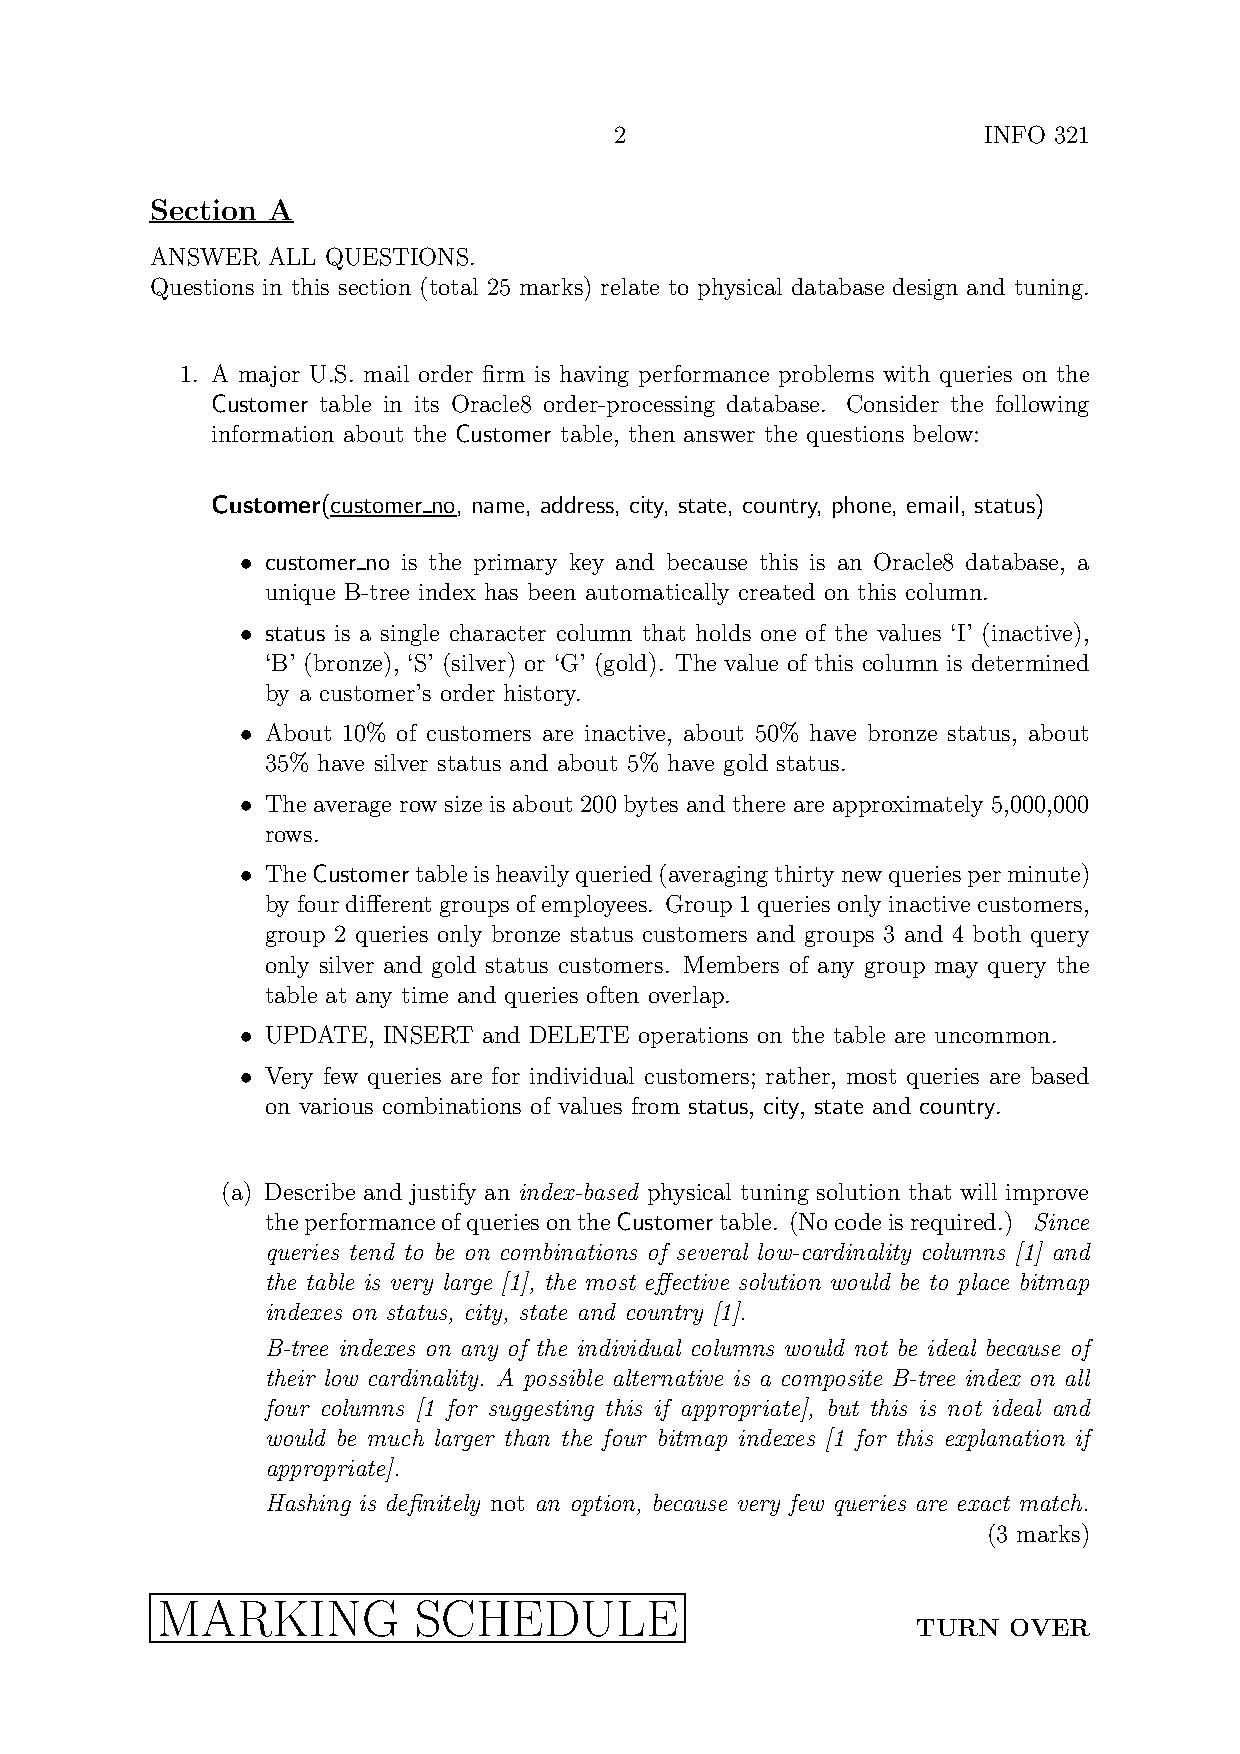
\includegraphics[bb=0 -57 596 785,scale=0.28]{eg2-2}}
% 	\hfill
% 	\fbox{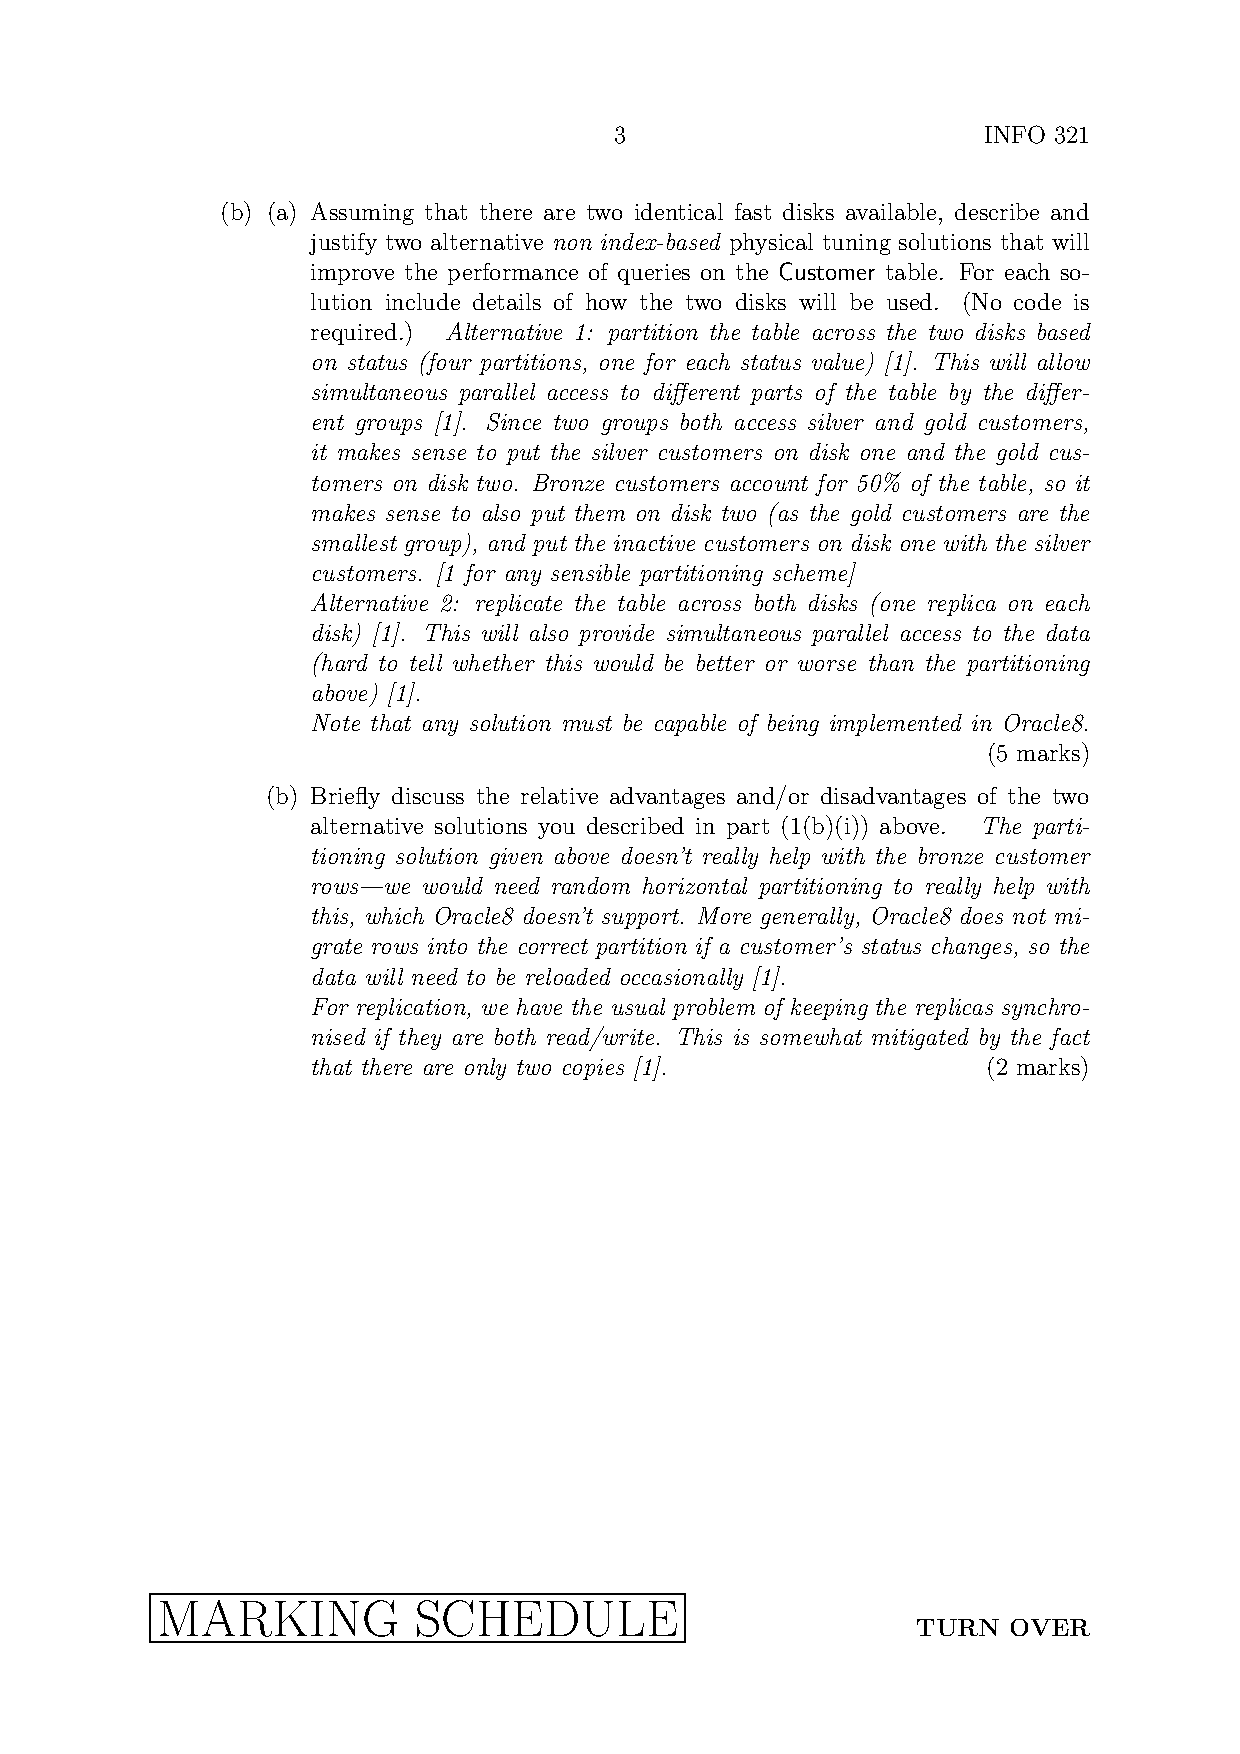
\includegraphics[bb=0 -57 596 785,scale=0.28]{eg2-3}}
% 
% 	\bigskip
% 	
% 	\fbox{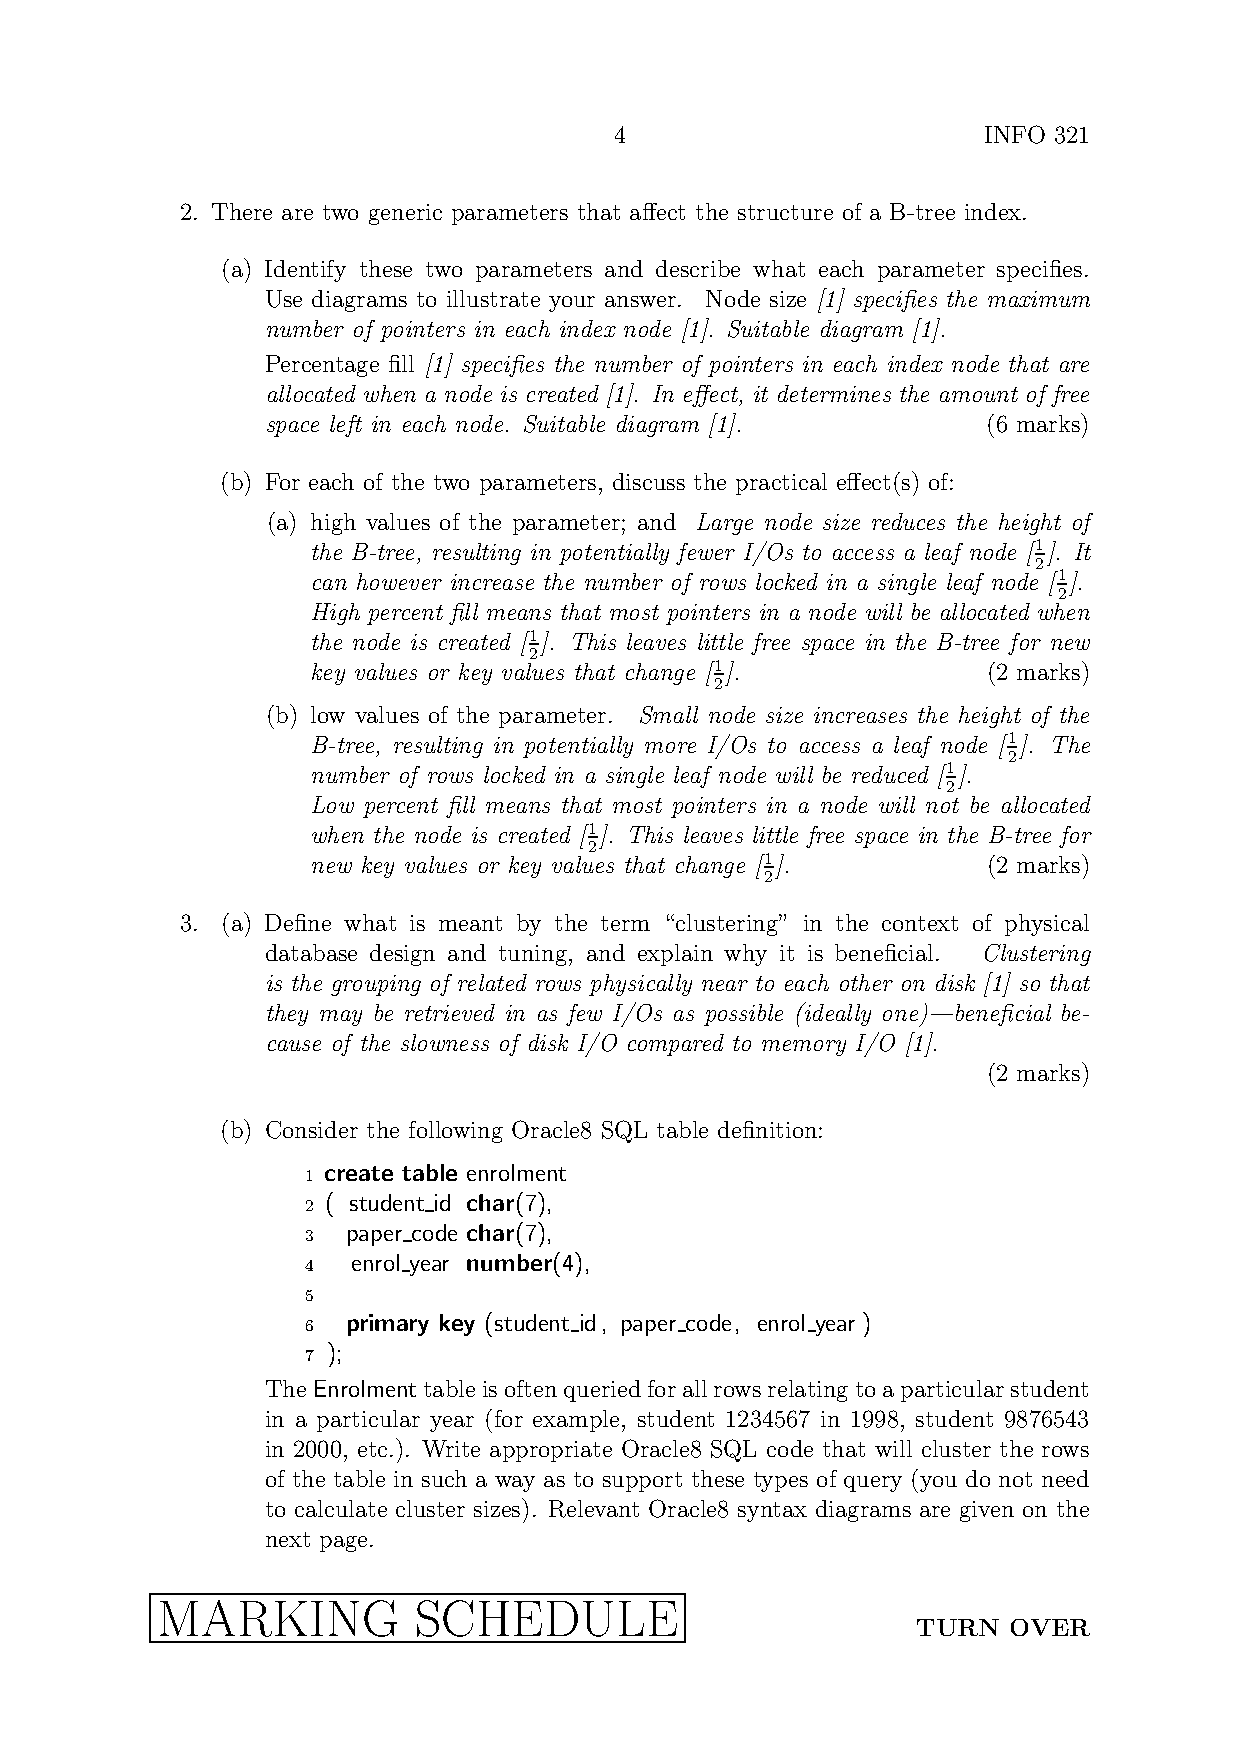
\includegraphics[bb=0 -57 596 785,scale=0.28]{eg2-4}}
% 	\hfill
% 	\fbox{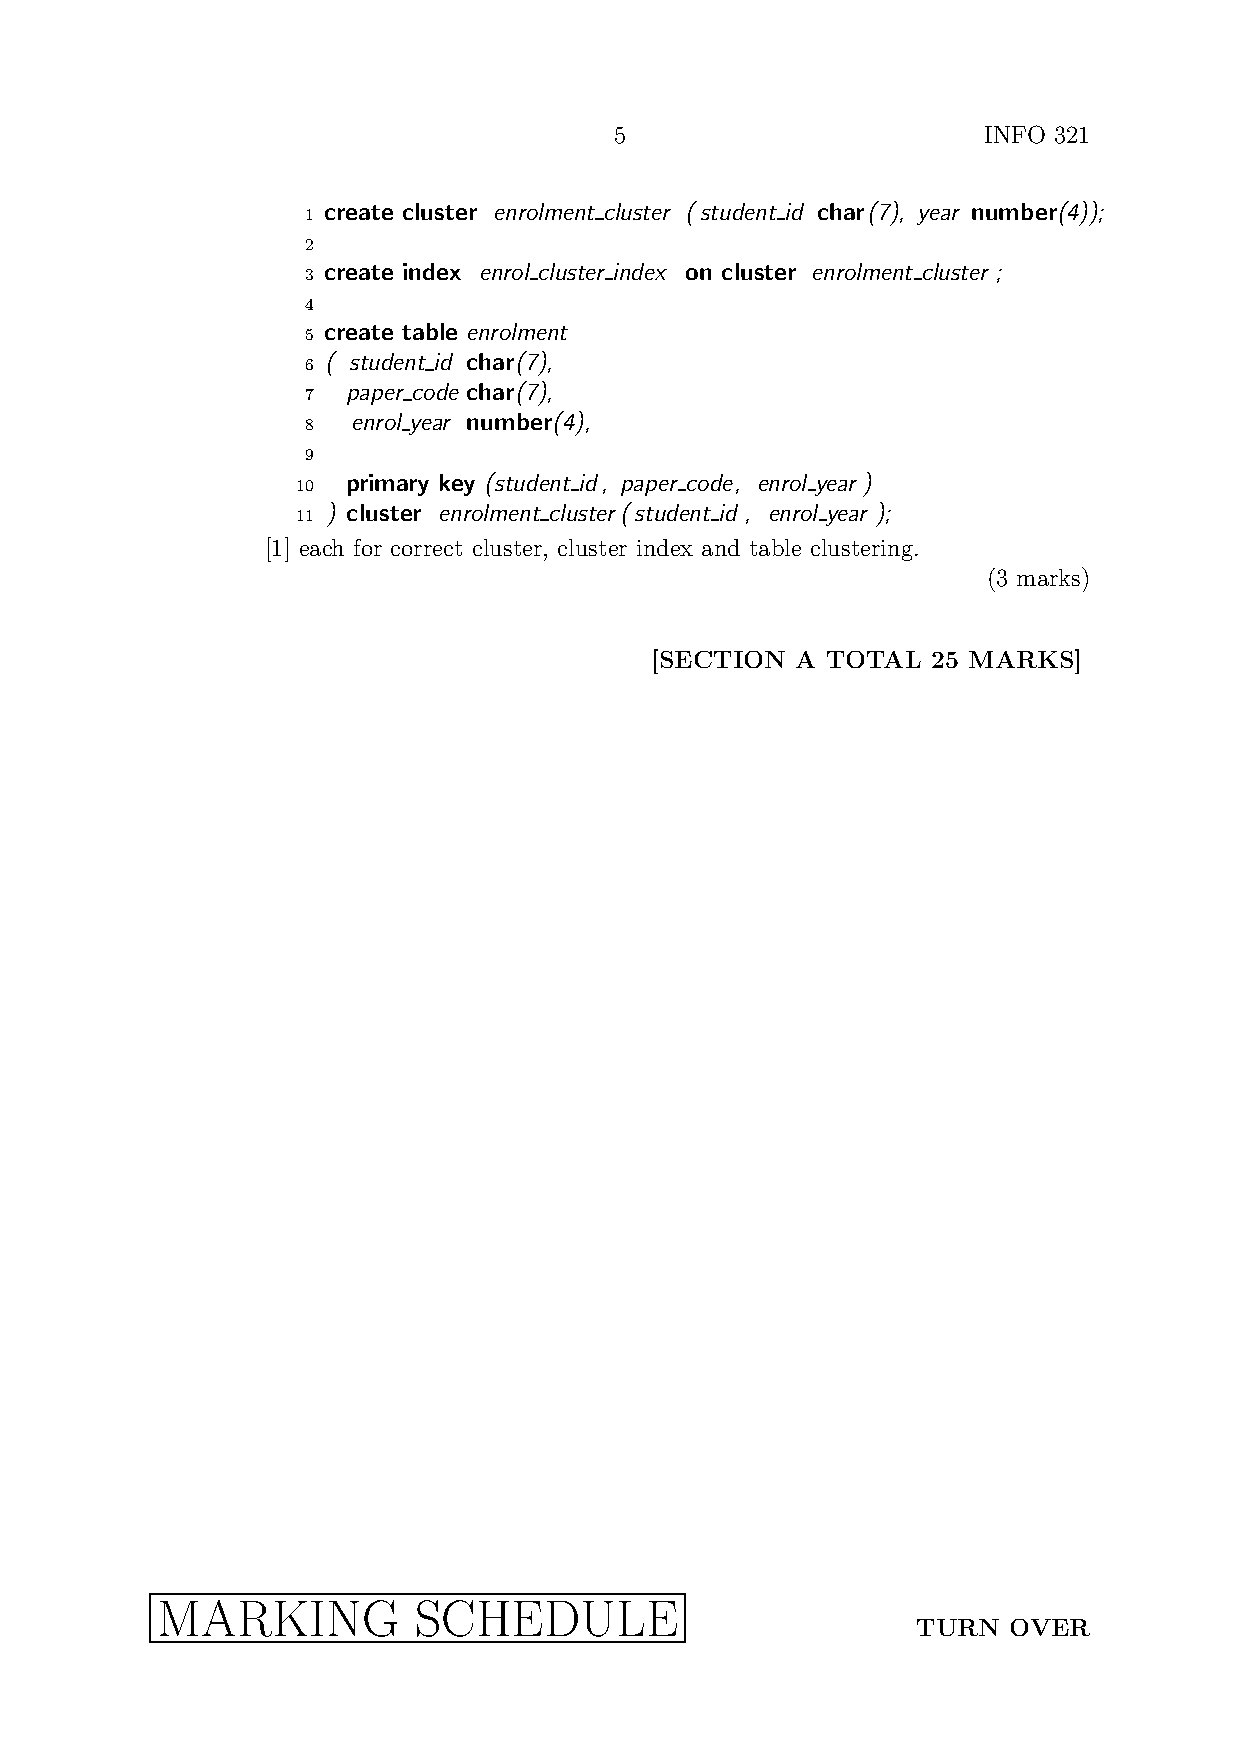
\includegraphics[bb=0 -57 596 785,scale=0.28]{eg2-5}}
% 
% 	\caption{Output produced by \textsf{ouexam} when
% 			\textsf{markingschedule} is used.}
% 	\label{Fig.Example2}
% \end{figure}
% 
% 
% \StopEventually{}
% 
% \changes{2.0}{2002/01/10}{NJS Revamped and tided up documentation and code.}
% 
% \section{The code}
% 
% \subsection{Preamble}
% 
%    \begin{macrocode}
\NeedsTeXFormat{LaTeX2e}[1998/06/01]
\ProvidesClass{ouexam}[\ouexamshortdate\space %
                           v\ouexamversion\space Otago %
                           University examination paper]
%    \end{macrocode}
% 
% \begin{macro}{\@unsupported}
% \changes{2.0}{2002/01/10}{NJS New \cs{@unsupported} macro.}
% This macro is used to handle documents written for older versions of
% \textsf{ouexam}. All obsolete macros map to this macro, which prints out an
% appropriate error message. It needs to be defined early because it is used
% to trap use of the obsolete \textsf{multichoice} class option.
%
%    \begin{macrocode}
\def\@unsupported#1{\ClassError{ouexam}{INCOMPATIBLE (#1): this %
  document was written for an earlier version of ouexam and is %
  not compatible with ouexam v\ouexamversion\space Please use ouexam %
  v1.2 or earlier to process this document. Version 1.2 can be %
  downloaded from the same location as version\space\ouexamversion}}
%    \end{macrocode}
% \end{macro}
%
% \begin{macro}{multichoice}
% \changes{1.1}{1999/04/20}{NJS New \textsf{multichoice} class option.}
% \changes{2.0}{2000/09/04}{NJS Removed support for \textsf{multichoice} option.}
% The \textsf{multichoice} class option is no longer supported, but rather than
% just breaking older documents, we can at least try to present a reasonable
% error message.
%
%    \begin{macrocode}
\DeclareOption{multichoice}{%
  \OptionNotUsed\@unsupported{multichoice class option}%
}
%    \end{macrocode}
% \end{macro}
%
% \begin{macro}{twoside}
% \changes{1.1}{1999/04/20}{NJS Turned off \textsf{twoside} option.}
% This document class is based on the \textsf{article} class and accepts any of
% the options accepted by \textsf{article}. The \textsf{twoside} option does
% not really make sense, however---all Otago examination papers are printed
% single-sided anyway, and the format is such that two-sided printing would
% look no different. The \textsf{twoside} option is therefore not used in this
% class.
%
%    \begin{macrocode}
\DeclareOption{twoside}{\OptionNotUsed}
%    \end{macrocode}
% \end{macro}
%
% \begin{macro}{draft}
% \changes{2.0}{2001/05/15}{NJS New \textsf{draft} class option.}
% \begin{macro}{\if@draft}
% \changes{2.0}{2001/05/15}{NJS New switch for \textsf{draft}.}
% The \textsf{draft} option determines whether the examination is to be printed
% in draft mode (default off). The \cs{if@draft} switch is used to determine
% whether this is in effect (default false). Draft mode has the usual effects
% that you would expect for draft mode in the \textsf{article} class, plus
% \fbox{DRAFT} is printed in the header of every page.
%
%    \begin{macrocode}
\newif\if@draft \@draftfalse
\DeclareOption{draft}{\@drafttrue}
% does this need to be passed to the article class?
%    \end{macrocode}
% 
% Note that if you use the \textsf{graphicx} package and turn on the
% \textsf{draft} option in \textsf{ouexam}, all included graphics will
% be drawn in draft mode unless you specify the |draft=false| option to the
% \cs{includegraphics} macro. The amount of effort required to fix what is
% a relatively small issue isn't really worth it, so this will not change.
% \end{macro}
% \end{macro}
% 
% \begin{macro}{markingschedule}
% \changes{2.0}{2000/09/05}{NJS New \textsf{markingschedule} class option.}
% \begin{macro}{\if@markingschedule}
% \changes{2.0}{2000/09/05}{NJS New switch for \textsf{markingschedule}.}
% The \textsf{markingschedule} option determines whether marking schedule
% information is printed in addition to the questions (default off). The
% \cs{if@markingschedule} switch is used to determine whether this is in effect
% (default false).
%
%    \begin{macrocode}
\newif\if@markingschedule \@markingschedulefalse
\DeclareOption{markingschedule}{\@markingscheduletrue}
%    \end{macrocode}
% \end{macro}
% \end{macro}
% 
% All other options are passed directly to the \textsf{article} class:
%
%    \begin{macrocode}
\DeclareOption*{\PassOptionsToClass{\CurrentOption}{article}}
\ProcessOptions
%    \end{macrocode}
%
% \changes{1.1}{1999/04/20}{NJS Changed default point size to 12pt.}
% The defaults for this class are \textsf{onecolumn}, \textsf{oneside},
% \textsf{a4paper} and \textsf{12pt}. The font size is the only one that might
% need to change.
%
%    \begin{macrocode}
\LoadClass[onecolumn,oneside,a4paper,12pt]{article}
%    \end{macrocode}
% 
% 
% \subsection{Required packages}
% 
% \changes{2.0}{2001/05/08}{NJS Removed requirement for \textsf{calc} and
% \textsf{ifthen} packages.}
% The only required package is the \textsf{verbatim} package, which is used
% to implement the \textsf{marking} environment:
%
%    \begin{macrocode}
\RequirePackage{verbatim}
%    \end{macrocode}
%
% 
% \subsection{Page setup}
% 
% \begin{macro}{\oddsidemargin}
% \begin{macro}{\topmargin}
% \begin{macro}{\textwidth}
% \begin{macro}{\textheight}
% A4 paper is assumed (since this class is intended only for Otago examination
% papers, this seems a reasonable assumption). The margins are top and bottom
% 2cm, left and right 2.54cm (1in).
%
%    \begin{macrocode}
\setlength{\oddsidemargin}{0cm}
\setlength{\topmargin}{-0.54cm}
\setlength{\textwidth}{15.92cm}
\setlength{\textheight}{25.7cm}
\advance\textheight by-\headheight
\advance\textheight by-\headsep
\advance\textheight by-\footskip
%    \end{macrocode}
% \end{macro}
% \end{macro}
% \end{macro}
% \end{macro}
% 
% 
% \subsection{Page styles}\label{pagestyles}
%
% \changes{2.0}{2001/05/17}{NJS Added support to page styles for \textsf{draft}
% and \textsf{markingschedule} class options.}
% \changes{2.0}{2002/01/15}{NJS Fixed headers so that the page number is always
% centered.}
% \changes{2.1.1}{2006/08/21}{NJS Updated \textsf{lastpage} style to display
% ``\textbf{END}''.}
%
% \begin{macro}{\ps@plain}
% The \textsf{plain} page style is based on that in the \textsf{article} class,
% and produces pages with the page number centered at the top, the paper number
% in the top right corner and the text ``\textbf{TURN OVER}'' in the bottom
% right. If semester information is specified, this is included in parentheses
% after the paper code, for example, ``COMP 101 (Semester Two)''.
%    \begin{macrocode}
\def\ps@plain{%
  \def\@oddhead{%
%    \end{macrocode}
% Note that we have to get a bit clever to ensure that the page number is
% properly centered in the page header. The naive solution is just to use
% \cs{hfill}s, but this will cause the page number to shift around depending on
% the length of \cs{@pnumber}. Piet van Oostrum's \textsf{fancyhdr} package will
% do this for us, but it seems a bit of overkill to require this package merely
% so that we can ensure that the page number remains centered. Instead, we've
% borrowed the relevant technique from that class, which draws the left, centre
% and right bits of the header as three overlapping boxes. You just have to be
% careful that the value of \cs{@pnumber} isn't so long that it overwrites the
% page number.
%    \begin{macrocode}
    \rlap{\parbox[b]{\columnwidth}{\raggedright\@draft\strut}}\hfill%
    \parbox[b]{\columnwidth}{\centering\textrm{\thepage}\strut}\hfill%
    \llap{\parbox[b]{\columnwidth}{\raggedleft\@pnumber%
      \ifx\@semester\@empty\else\ (\@semester)\fi\strut}}}%
  \let\@evenhead\@oddhead%
  \def\@oddfoot{\@markingschedule\hfill\textbf{TURN OVER}}%
  \let\@evenfoot\@oddfoot%
}
%    \end{macrocode}
% \end{macro}
% \textsf{plain} is the default page style:
%    \begin{macrocode}
\pagestyle{plain}
%    \end{macrocode}
% 
% \begin{macro}{\ps@lastpage}
% The \textsf{lastpage} page style is similar to \textsf{plain}, but with
% ``\textbf{END}'' instead of ``\textbf{TURN OVER}'':
%    \begin{macrocode}
\def\ps@lastpage{%
  \def\@oddhead{%
    \rlap{\parbox[b]{\columnwidth}{\raggedright\@draft\strut}}\hfill%
    \parbox[b]{\columnwidth}{\centering\textrm{\thepage}\strut}\hfill%
    \llap{\parbox[b]{\columnwidth}{\raggedleft\@pnumber%
      \ifx\@semester\@empty\else\ (\@semester)\fi\strut}}}%
  \let\@evenhead\@oddhead%
  \def\@oddfoot{\@markingschedule\hfill\textbf{END}}%
  \let\@evenfoot\@oddfoot%
}
%    \end{macrocode}
% \end{macro}
% \textsf{lastpage} should be automatically applied to the last page of the
% document:
%    \begin{macrocode}
\AtEndDocument{\thispagestyle{lastpage}}
%    \end{macrocode}
% 
% \begin{macro}{\ps@titlepage}
% The \textsf{titlepage} page style is similar to \textsf{plain}, but without
% the header.
%    \begin{macrocode}
\def\ps@titlepage{%
  \def\@oddhead{\@draft}%
  \let\@evenhead\@oddhead%
  \def\@oddfoot{\@markingschedule\hfill\textbf{TURN OVER}}%
  \let\@evenfoot\@oddfoot%
}
%    \end{macrocode}
% \end{macro}
% 
% 
% \subsection{Various counters}
% 
% Earlier versions of \textsf{ouexam} used the \textsf{enumerate}
% environment to build questions, which meant that special counters were not
% required. This version of the class, however, uses a different mechanism for
% building questions, so we need to define custom counters for several things.
% 
% \begin{macro}{question}
% \begin{macro}{subquestion}
% \changes{2.0}{2000/09/11}{NJS New \texttt{subquestion} counter.}
% \changes{2.0.1}{2000/04/30}{NJS Removed prefixed question number from
% \cs{labelsubquestion} macro so that references now print as just ``(a)''
% instead of ``1(a)''.}
% \begin{macro}{subsubquestion}
% \changes{2.0}{2000/09/11}{NJS New \texttt{subsubquestion} counter.}
% \changes{2.0.1}{2000/04/30}{NJS The \texttt{subsubquestion} was incorrectly
% printing as ``(a)'' rather than ``(i)''. Fixed.}
% \changes{2.0.1}{2000/04/30}{NJS Removed prefixed question numbers from
% \cs{labelsubsubquestion} macro so that references now print as just ``(i)''
% instead of ``1(a)(i)''.}
% First, we define three counters for the three possible levels of question:
% top-level question, second-level sub-question or third-level sub-sub-question:
%    \begin{macrocode}
\newcounter{question}
\newcounter{subquestion}[question]
\newcounter{subsubquestion}[subquestion]
%    \end{macrocode}
% The three question levels are numbered as 1., (a) and (i) respectively, so we
% also need to redefine the associated \cs{the} and \cs{label} macros
% appropriately:
%    \begin{macrocode}
\renewcommand{\thequestion}{\arabic{question}}
\newcommand{\labelquestion}{\hfil\arabic{question}.}

\renewcommand{\thesubquestion}{(\alph{subquestion})}
\newcommand{\labelsubquestion}{\hfil(\alph{subquestion})}

\renewcommand{\thesubsubquestion}{(\roman{subsubquestion})}
\newcommand{\labelsubsubquestion}{\hfil(\roman{subsubquestion})}
%    \end{macrocode}
% \end{macro}
% \end{macro}
% \end{macro}
% 
% \begin{macro}{examexpected}
% \changes{2.0}{2000/09/11}{NJS New \texttt{examexpected} counter.}
% The |examexpected| counter stores the total expected number of marks for the
% examination, and defaults to 100:
%    \begin{macrocode}
\newcounter{examexpected}
\setcounter{examexpected}{100}
%    \end{macrocode}
% \end{macro}
% \begin{macro}{examoutof}
% \changes{2.0}{2000/09/11}{NJS New \texttt{examoutof} macro.}
% To specify that an examination is out of some number of marks other than
% 100, use the \cs{examoutof} macro to set the value:
%    \begin{macrocode}
\newcommand{\examoutof}[1]{\setcounter{examexpected}{#1}}
%    \end{macrocode}
% \end{macro}
% 
% \begin{macro}{sectexpected}
% \changes{2.0}{2002/01/09}{NJS New \cs{sectexpected} counter.}
% \begin{macro}{qexpected}
% \changes{2.0}{2000/09/11}{NJS New \cs{qexpected} counter.}
% \begin{macro}{subqexpected}
% \changes{2.0}{2000/09/11}{NJS New \texttt{subqexpected} counter.}
% \begin{macro}{subsubqexpected}
% \changes{2.0}{2000/09/11}{NJS New \texttt{subsubqexpected} counter.}
% The next four counters perform the same function as the |examexpected| counter
% for sections, questions, sub-questions and sub-sub-questions respectively. No
% macros are required to set these values as they are set automatically by the
% question-building environments.
% 
%    \begin{macrocode}
\newcounter{sectexpected}
\newcounter{qexpected}
\newcounter{subqexpected}
\newcounter{subsubqexpected}
%    \end{macrocode}
% \end{macro}
% \end{macro}
% \end{macro}
% \end{macro}
% 
% \begin{macro}{lastexpected}
% \changes{2.0}{2000/09/11}{NJS New \texttt{lastexpected} counter.}
% The |lastexpected| counter records the expected marks total for the last
% question. This will eventually be used to verify that the marks total for a
% marking schedule equals the marks total for the corresponding question, but
% this hasn't been implemented yet.
% 
%    \begin{macrocode}
\newcounter{lastexpected}
%    \end{macrocode}
% \end{macro}
% 
% \begin{macro}{examrunning}
% \changes{2.0}{2000/09/11}{NJS New \texttt{examrunning} counter.}
% \begin{macro}{sectrunning}
% \changes{2.0}{2002/01/09}{NJS New \texttt{sectrunning} counter.}
% \begin{macro}{qrunning}
% \changes{2.0}{2000/09/11}{NJS New \texttt{qrunning} counter.}
% \begin{macro}{subqrunning}
% \changes{2.0}{2000/09/11}{NJS New \texttt{subqrunning} counter.}
% These four counters keep track of the running total of marks for the
% current examination, section, question and subquestion respectively. This
% is later compared against the corresponding expected total. A running total
% is not needed for sub-sub-questions because they do not have sub-parts. The
% |qrunning| and |subqrunning| counters are reset when the associated
% question counters are incremented.
% 
%    \begin{macrocode}
\newcounter{examrunning}
\setcounter{examrunning}{0}
\newcounter{sectrunning}
\newcounter{qrunning}[question]
\newcounter{subqrunning}[subquestion]
%    \end{macrocode}
% \end{macro}
% \end{macro}
% \end{macro}
% \end{macro}
% 
% \begin{macro}{hassubs}
% \changes{2.0}{2000/09/11}{NJS New \texttt{hassubs} counter.}
% \begin{macro}{hassubsubs}
% \changes{2.0}{2000/09/11}{NJS New \texttt{hassubsubs} counter.}
% These two counters are used to track whether questions and
% sub-questions have sub-parts. Counters are used rather than booleans because
% counters are set globally and booleans are not (or at least do not appear to
% be). Both counters reset when the associated question counters are
% incremented.
% 
%    \begin{macrocode}
\newcounter{hassubs}[question]
\newcounter{hassubsubs}[subquestion]
%    \end{macrocode}
% \end{macro}
% \end{macro}
% 
% At the end of the document, check that the running total of marks for the
% examination matches what we were expecting:
% 
%    \begin{macrocode}
\AtEndDocument{%
  \ifnum\theexamexpected=\theexamrunning%
  \else\ClassWarning{ouexam}{actual number of marks for exam %
      (\theexamrunning) does not match expected number of marks %
      (\theexamexpected)}%
  \fi%
}
%    \end{macrocode}
% 
% \begin{macro}{xsection}
% \changes{2.0}{2002/01/29}{NJS New \texttt{xsection} counter.}
% Finally, we set up a counter for the section ``number'' and define it so
% that it prints out as an upper case letter rather than a number. We could
% just redefine the |section| counter, but that interferes with the section
% numbering in the documentation, and we can't have that, can we? |:)|
% 
%    \begin{macrocode}
\newcounter{xsection}
\setcounter{xsection}{0}
\renewcommand{\thexsection}{\Alph{xsection}}
%    \end{macrocode}
% \end{macro}
%
% 
% \subsection{Question-building environments and associated items}
% 
% \changes{2.0}{2000/09/11}{NJS \textsf{question} environment no longer a
% redefinition of \textsf{enumerate}.}
% \changes{2.0}{2001/05/15}{NJS Added penalty handling to ensure correct
% placement of marks in output.}
% \changes{2.0}{2001/05/15}{NJS Total marks for a question are now printed only
% if the question has no sub-questions.}
% \begin{environment}{question}
% The \textsf{question} environment specifies a top-level question, and produces
% questions numbered in the form ``1.'', ``2.'', etc. It has one mandatory
% argument, the number of marks allocated to the question, which is used to
% initialise the |qexpected| counter\footnote{If it were not for the fact that
% you can only refer to environment arguments in the environment preamble, the
% \texttt{qexpected} counter would be unnecessary.}. If the argument is left
% empty, default to zero for the number of marks:
% 
%    \begin{macrocode}
\newenvironment{question}[1]{%
  \def\@nummarks{#1}%
  \ifx\@nummarks\@empty\setcounter{qexpected}{0}%
  \else\setcounter{qexpected}{#1}\fi%
%    \end{macrocode}
% 
% For each top-level question, we increment the |question| counter, which also
% resets the |hassubs| and |qrunning| counters to zero:
%    \begin{macrocode}
  \refstepcounter{question}%
%    \end{macrocode}
% The question itself is built using a single-item \textsf{list} environment.
%    \begin{macrocode}
  \begin{list}{\labelquestion}{\settowidth{\labelwidth}{88.}}%
    \item \ignorespaces%
%    \end{macrocode}
% 
% When the environment closes, the following things happen:
% \begin{enumerate}
% 	\item If the question has no sub-questions, the value of the |qexpected|
% 	counter is added to |examrunning| and |sectrunning|, and both |qrunning|
% 	and |lastexpected| are set to the value of |qexpected|.
% 
%    \begin{macrocode}
}{%
    \ifnum\thehassubs=0%
      \addtocounter{examrunning}{\value{qexpected}}%
      \addtocounter{sectrunning}{\value{qexpected}}%
      \setcounter{qrunning}{\value{qexpected}}%
%    \end{macrocode}
% 
% 	The total number of marks for the question is then printed right-justified
% 	on the line as ``(\emph{m} marks)'' where \emph{m} is the value of the
% 	|qrunning| counter. The environment determines whether to print ``mark'' or
% 	``marks'' automatically, and figures out whether the number of marks will fit
% 	on the last line of the question or needs to be placed on the next line.
% 	The code for handling the line breaking is derived from an example on page
% 	106 of \emph{The \TeX{}book}:
% 
%    \begin{macrocode}
      \unskip\nobreak\hfil\penalty50\hskip2em\hbox{}\nobreak%
      \hfil(\theqrunning~\ifnum\theqrunning=1 mark\else marks\fi)%
      \parfillskip=0pt \finalhyphendemerits=0 \par%
%    \end{macrocode}
% 
% 	\item If the question \emph{does} have sub-questions, then |qrunning|,
% 	|examrunning| and |sectrunning| have already been set by the various
% 	sub-environments. The value of |qrunning| is then compared with
% 	|qexpected|, and a warning is raised if they do not match. The total number
% 	of marks for the question is \emph{not} printed in this case.
% 
%    \begin{macrocode}
    \else%
      \ifnum\theqrunning=\theqexpected%
      \else\ClassWarning{ouexam}{actual mark (\theqrunning) for %
          question \thequestion\space doesn't match expected mark %
          (\theqexpected)}%
      \fi%
    \fi%
%    \end{macrocode}
% 
% 	\item |lastexpected| is set to the value of |qexpected| so it can be used
% 	in any subsequent \textsf{marking} environment.
% 
%    \begin{macrocode}
    \setcounter{lastexpected}{\value{qexpected}}%
  \end{list}%
}
%    \end{macrocode}
% 
% \end{enumerate}
% \end{environment}
% 
% \begin{environment}{subquestion}
% \changes{2.0}{2000/09/11}{NJS \textsf{subquestion} environment no longer a
% redefinition of \textsf{enumerate}.}
% \changes{2.0}{2001/05/13}{NJS Added penalty handling to ensure correct placement
% of marks in output.}
% The \textsf{subquestion} environment is the analogue of \textsf{question} for
% sub-questions. On initialisation, it sets |subqexpected| to the value of the
% mandatory argument (defaulting to zero if the argument is empty), increments
% the |hassubs| counter so that the enclosing \textsf{question} environment can
% react appropriately, increments |subquestion| (thus resetting |hassubsubs| and
% |subqrunning| to zero) and opens a single-item list with numbering of the form
% ``(a)'', ``(b)'', etc.
% 
%    \begin{macrocode}
\newenvironment{subquestion}[1]{%
  \def\@nummarks{#1}%
  \ifx\@nummarks\@empty\setcounter{subqexpected}{0}%
  \else\setcounter{subqexpected}{#1}\fi%
  \setcounter{subqexpected}{#1}%
  \addtocounter{hassubs}{1}%
  \refstepcounter{subquestion}%
  \begin{list}{\labelsubquestion}{\settowidth{\labelwidth}{(m)}}%
    \item \ignorespaces%
}{%
%    \end{macrocode}
% 
% When the environment closes, if performs similar checks to the
% \textsf{question} environment. If the sub-question has no sub-sub-questions,
% the value of |subqexpected| is added to |qrunning| and |sectrunning|:
% 
%    \begin{macrocode}
    \ifnum\thehassubsubs=0%
      \addtocounter{examrunning}{\value{subqexpected}}%
      \addtocounter{sectrunning}{\value{subqexpected}}%
      \addtocounter{qrunning}{\value{subqexpected}}%
      \setcounter{subqrunning}{\value{subqexpected}}%
%    \end{macrocode}
% Then the number of marks for the sub-question are typeset in a similar manner
% to the \textsf{question} environment:
%    \begin{macrocode}
      \unskip\nobreak\hfil\penalty50\hskip2em\hbox{}\nobreak%
      \hfil(\thesubqrunning~\ifnum\thesubqrunning=1 mark\else marks\fi)%
      \parfillskip=0pt \finalhyphendemerits=0 \par%
%    \end{macrocode}
% 
% If the sub-question \emph{does} have sub-sub-questions, check the running total
% against the expected number and raise an error if they don't match.
%    \begin{macrocode}
    \else%
      \ifnum\thesubqrunning=\thesubqexpected%
      \else\ClassWarning{ouexam}{actual mark (\thesubqrunning) for %
          question \thesubquestion\space doesn't match expected mark %
          (\thesubqexpected)}%
      \fi%
    \fi%
%    \end{macrocode}
% Finally, set |lastexpected| to the value of |qexpected| so it can be used
% in any subsequent \textsf{marking} environment.
%    \begin{macrocode}
    \setcounter{lastexpected}{\value{subqexpected}}%
  \end{list}%
}
%    \end{macrocode}
% \end{environment}
% 
% \begin{environment}{subsubquestion}
% \changes{2.0}{2000/09/11}{NJS \textsf{subsubquestion} environment no longer a
% redefinition of \textsf{enumerate}.}
% \changes{2.0}{2001/05/13}{NJS Added penalty handling to ensure correct placement
% of marks in output.}
% This is similar to both \textsf{question} and \textsf{subquestion}, and
% generates an appropriately numbered sub-sub-question (``(i)'', ``(ii)'', etc.).
%    \begin{macrocode}
\newenvironment{subsubquestion}[1]{%
  \def\@nummarks{#1}%
  \ifx\@nummarks\@empty\setcounter{subsubqexpected}{0}%
  \else\setcounter{subsubqexpected}{#1}\fi%
%    \end{macrocode}
% Increment |hassubsubs| so that the enclosing \textsf{subquestion} environment
% can react appropriately:
%    \begin{macrocode}
  \addtocounter{hassubsubs}{1}%
  \refstepcounter{subsubquestion}%
  \begin{list}{\labelsubsubquestion}{\settowidth{\labelwidth}{(viii)}}%
    \item \ignorespaces%
}{%
%    \end{macrocode}
% 
% Closing this environment is a bit simpler than the previous two because we
% don't need to check whether the sub-sub-question has any sub-components (this
% never happens). All we have to do is set the appropriate counters and typeset
% the number of marks.
% 
%    \begin{macrocode}
    \addtocounter{examrunning}{\value{subsubqexpected}}%
    \addtocounter{sectrunning}{\value{subsubqexpected}}%
    \addtocounter{qrunning}{\value{subsubqexpected}}%
    \addtocounter{subqrunning}{\value{subsubqexpected}}%
    \setcounter{lastexpected}{\value{subsubqexpected}}%
    \unskip\nobreak\hfil\penalty50\hskip2em\hbox{}\nobreak%
    \hfil(\thesubsubqexpected~\ifnum\thesubsubqexpected=1 mark%
                              \else marks\fi)%
    \parfillskip=0pt \finalhyphendemerits=0 \par%
  \end{list}%
}
%    \end{macrocode}
% \end{environment}
% 
% Note that none of these three environments check whether they are correctly
% nested (i.e., \textsf{subsubquestion} within \textsf{subquestion} within
% \textsf{question}).
% 
% 
% \subsection{Draft examination printing}
% 
% \begin{macro}{\@marking}
% \changes{2.0}{2001/05/17}{NJS New \cs{@draft} macro.}
% Specifying the \textsf{draft} option causes \textsf{ouexam} to print
% \fbox{DRAFT} in large letters in the header of every page. This is drawn by
% the \cs{@draft} macro, which is included in the page header definition of
% all the page styles for this class (see
% \hyperref[pagestyles]{section~\ref*{pagestyles}}). \textbf{Note:} Because
% the \cs{@draft} macro is included in the page header, it will usually
% overflow the page boundaries, causing ``|Overfull \vbox|'' warnings. Note
% the extra set of braces to limit the scope of the \cs{Huge}.
% 
%    \begin{macrocode}
\if@draft\def\@draft{{\Huge\fbox{DRAFT}}}
\else\let\@draft\@empty
\fi
%    \end{macrocode}
% \end{macro}
% 
% 
% \subsection{Marking schedule information}
% 
% \begin{environment}{marking}
% \begin{macro}{\@markingschedule}
% \changes{1.2}{1999/10/26}{NJS New \textsf{marking} environment for including
% answers and/or marking schedule information.}
% \changes{2.0}{2000/09/11}{NJS Now prints ``MARKING SCHEDULE'' at the bottom
% of every page if the \textsf{markingschedule} class option is specified.}
% The \textsf{marking} environment allows the specification of marking
% schedule information in the same location as the questions. If the
% \textsf{markingschedule} class option is specified, marking schedule
% information is printed in italics. In addition, \fbox{MARKING SCHEDULE} is
% printed in large letters in the footer of every page. This is drawn by the
% \cs{@markingschedule} macro, which is included in the page footer
% definition of all the page styles for this class (see
% \hyperref[pagestyles]{section~\ref*{pagestyles}}). Note the extra set of
% braces to limit the scope of the \cs{Huge}.
% 
%    \begin{macrocode}
\if@markingschedule
  \newenvironment{marking}{\itshape}{\normalfont}
  \def\@markingschedule{{\Huge\fbox{MARKING SCHEDULE}}}
\else
%    \end{macrocode}
% 
% Normally \textsf{marking} just maps to the \textsf{comment} environment from
% Rainer Sch\"{o}pf's \textsf{verbatim} package, i.e., marking information is not
% printed:
% 
%    \begin{macrocode}
  \let\marking\comment
  \let\endmarking\endcomment
  \let\@markingschedule\@empty
\fi
%    \end{macrocode}
% \end{macro}
% \end{environment}
% 
% 
% \subsection{Section handling}
% 
% \changes{2.0}{2002/01/09}{NJS new \textsf{examsection} environment.}
% \changes{2.0}{2002/01/09}{NJS New \cs{@defsecinst} macro.}
% \begin{environment}{examsection}
% \begin{macro}{\@defsecinst}
% The \textsf{examsection} environment specifies a major section of an
% examination paper. Sections are sequentially numbered ``A'', ``B'', etc. The
% environment has three arguments:
% 
% \begin{enumerate}
% 	\item The expected number of marks for the section.
% 
% 	\item The instructions for this section. This defaults to ``ANSWER ALL
%	QUESTIONS.'' if left blank. To change the default text, redefine the
%	\cs{@defsecinst} macro.
%    \begin{macrocode}
\def\@defsecinst{ANSWER ALL QUESTIONS.}
%    \end{macrocode}
% 
% 	\item A description of the contents of the section which may be left blank.
% \end{enumerate}
% 
%    \begin{macrocode}
\newenvironment{examsection}[3]{%
%    \end{macrocode}
% Every section begins on a new page.
%    \begin{macrocode}
  \newpage%
%    \end{macrocode}
% If the argument for the number of marks is left empty, default to zero.
%    \begin{macrocode}
  \def\@nummarks{#1}%
  \ifx\@nummarks\@empty\setcounter{sectexpected}{0}%
  \else\setcounter{sectexpected}{#1}\fi%
  \refstepcounter{xsection}%
  \setcounter{sectrunning}{0}%
%    \end{macrocode}
% The section title is formatted as ``\textbf{\underline{Section A}}'', in
% \cs{large} size.
%    \begin{macrocode}
  {\large\noindent\textbf{\underline{Section~\thexsection}}}%
  \\[0.5\baselineskip]%
  \def\@usersecinst{#2}%
  \ifx\@usersecinst\@empty\@defsecinst\else\@usersecinst\fi\par%
  \def\@usersectopic{#3}%
  \ifx\@usersectopic\@empty\else\par\noindent\@usersectopic\fi \\%
}{%
%    \end{macrocode}
% 
% When the environment closes, the value of |sectrunning| is compared against
% |sectexpected|, and a warning is raised if they do not match. The total number
% marks for the section is printed in the form ``\textbf{[SECTION A TOTAL
% \emph{m} MARKS]}'' where \emph{m} is the value of |sectrunning|.
% 
%    \begin{macrocode}
  \ifnum\thesectrunning=\thesectexpected%
  \else\ClassWarning{ouexam}{actual mark (\thesectrunning) for section %
      \thexsection\space doesn't match expected mark (\thesectexpected)}%
  \fi%
  \bigskip\hfill\textbf{[SECTION \thexsection\ TOTAL %
                              \thesectrunning\ MARKS]}%
}
%    \end{macrocode}
% \end{macro}
% \end{environment}
%
% \begin{macro}{\newsection}
% \textbf{[DEPRECATED]} The \cs{newsection} macro generates a new examination
% section, appropriately numbered. The optional argument contains instructions
% for answering the questions in the new section, and defaults to ``ANSWER ALL
% QUESTIONS''. This macro is included only for backwards compatibility with
% previous versions. The \textsf{examsection} environment replaces this macro
% and should be used in new documents. This macro will eventually be deleted.
%    \begin{macrocode}
\newcommand{\newsection}[1][ANSWER ALL QUESTIONS.]{%
  \ClassWarning{ouexam}{DEPRECATED: The \protect\newsection\space %
      macro is deprecated; use the examsection environment instead}%
%    \end{macrocode}
% Every section begins on a new page.
%    \begin{macrocode}
  \newpage%
  \refstepcounter{xsection}%
%    \end{macrocode}
% The section title is formatted as ``\textbf{\underline{Section A}}'', in
% \cs{large} size. Note that sections are ``numbered'' A, B, \ldots.
%    \begin{macrocode}
  {\large\noindent\textbf{\underline{Section~\thexsection}}}%
  \\[0.5\baselineskip]%
  #1%
}
%    \end{macrocode}
% \end{macro}
% 
% 
% \subsection{Title page generation}
% 
% \begin{macro}{\examyear}
% \begin{macro}{\@year}
% \changes{2.0.2}{2002/08/22}{NJS Put back \@eha at end of the \ClassError. Don't
% know what this does, but the macro crashes without it there.}
% The \cs{examyear} macro specifies the year in which the examination is being
% held. It redefines the \cs{@year} macro which is used in \cs{@maketitlepage}:
%    \begin{macrocode}
\newcommand{\examyear}[1]{\def\@year{#1}}
%    \end{macrocode}
% This macro is required:
%    \begin{macrocode}
\def\@year{%
  \ClassError{ouexam}{no \protect\examyear\space was specified}\@eha%
}
%    \end{macrocode}
% \end{macro}
% \end{macro}
% 
% \begin{macro}{\department}
% \begin{macro}{\@dept}
% \changes{2.0.2}{2002/08/22}{NJS Put back \@eha at end of the \ClassError. Don't
% know what this does, but the macro crashes without it there.}
% The \cs{department} macro specifies the name of the department, and is required.
% It redefines the \cs{@dept} macro which is used in \cs{@maketitlepage}:
%    \begin{macrocode}
\newcommand{\department}[1]{\def\@dept{#1}}
\def\@dept{%
  \ClassError{ouexam}{no \protect\department\space was specified}\@eha%
}
%    \end{macrocode}
% \end{macro}
% \end{macro}
% 
% \begin{macro}{\papernumber}
% \begin{macro}{\@pnumber}
% \changes{2.0.2}{2002/08/22}{NJS Put back \@eha at end of the \ClassError. Don't
% know what this does, but the macro crashes without it there.}
% The \cs{papernumber} macro specifies the paper number, and is required.
% It redefines the \cs{@pnumber} macro which is used in \cs{@maketitlepage}:
%    \begin{macrocode}
\newcommand{\papernumber}[1]{\def\@pnumber{#1}}
\def\@pnumber{%
  \ClassError{ouexam}{no \protect\papernumber\space was specified}\@eha%
}
%    \end{macrocode}
% \end{macro}
% \end{macro}
% 
% \begin{macro}{\papertitle}
% \begin{macro}{\@ptitle}
% \changes{2.0.2}{2002/08/22}{NJS Put back \@eha at end of the \ClassError. Don't
% know what this does, but the macro crashes without it there.}
% The \cs{papertitle} macro specifies the title of the paper, and is required.
% It redefines the \cs{@ptitle} macro which is used in \cs{@maketitlepage}:
%    \begin{macrocode}
\newcommand{\papertitle}[1]{\def\@ptitle{#1}}
\def\@ptitle{%
  \ClassError{ouexam}{no \protect\papertitle\space was specified}\@eha%
}
%    \end{macrocode}
% \end{macro}
% \end{macro}
% 
% \begin{macro}{\semester}
% \begin{macro}{\@semester}
% \changes{2.0.2}{2002/08/22}{NJS Added full-year support to \cs{semester}.}
% \changes{2.0}{2002/01/14}{NJS Rewrote \cs{semester} to support summer school
% and special exams.}
% The \cs{semester} macro specifies which semester the examination is for.
% Legal values for the argument are ``1'', ``2'', ``SS'' for summer school,
% ``FY'' for full-year or ``SP'' for a special examination---anything else is
% ignored.
%    \begin{macrocode}
\def\@ONE{1}
\def\@TWO{2}
\def\@SS{SS}
\def\@FY{FY}
\def\@SP{SP}
%    \end{macrocode}
% This macro redefines the \cs{@semester} macro which is used in
% \cs{@maketitlepage}:
%    \begin{macrocode}
\newcommand{\semester}[1]{%
  \def\@sem{#1}%
  \ifx\@sem\@ONE\def\@semester{Semester One}%
  \else\ifx\@sem\@TWO\def\@semester{Semester Two}%
  \else\ifx\@sem\@SS\def\@semester{Summer School}%
  \else\ifx\@sem\@FY\def\@semester{Full Year}%
  \else\ifx\@sem\@SP\def\@semester{Special Examination}%
  \else\ClassWarning{ouexam}{invalid value `#1' for %
    \protect\semester; valid values are `1', `2', `SS', %
    `FY' and `SP'. No semester information will be printed}%
  \fi\fi\fi\fi\fi%
}
%    \end{macrocode}
% \cs{semester} is optional---if you omit it or give it an invalid argument,
% \cs{@semester} remains empty.
%    \begin{macrocode}
\let\@semester\@empty
%    \end{macrocode}
% \end{macro}
% \end{macro}
% 
% \begin{macro}{\timeallowed}
% \begin{macro}{\@hours}
% The \cs{timeallowed} macro specifies the length of the examination in hours.
% It redefines the \cs{@hours} macro which is used in \cs{@maketitlepage}:
%    \begin{macrocode}
\newcommand{\timeallowed}[1]{\def\@hours{#1}}
%    \end{macrocode}
% \cs{timeallowed} is optional---if you omit it, \cs{@hours} defaults to ``3'':
%    \begin{macrocode}
\def\@hours{3}
%    \end{macrocode}
% \end{macro}
% \end{macro}
% 
% \begin{macro}{num.pages}
% \changes{1.1}{1999/04/20}{NJS Renamed label from \cs{page.last}.}
% There is no macro to specify the number of pages in the examination because
% it is done automatically by inserting a \cs{newlabel} that refers to the last
% page directly into the |.aux| file:
%    \begin{macrocode}
\AtEndDocument{%
  \immediate\write\@auxout{\string\newlabel{num.pages}{{}{\thepage}}}%
}
%    \end{macrocode}
% This label is then referenced in \cs{@maketitlepage}.
% \end{macro}
% 
% \begin{macro}{num.questions}
% \changes{1.1}{1999/04/20}{NJS New \cs{num.questions} label representing the
% number of questions.}
% Similarly, there is no macro to specify the number of questions in the
% examination. This is calculated using the same method as for the number of
% pages:
%    \begin{macrocode}
\AtEndDocument{%
  \immediate\write\@auxout{%
    \string\newlabel{num.questions}{{}{\thequestion}}%
  }%
}
%    \end{macrocode}
% \end{macro}
% 
% \begin{macro}{\instructions}
% \begin{macro}{\@instructions}
% The \cs{instructions} macro specifies instructions on how candidates should
% answer questions. It redefines the \cs{@instructions} macro that is used in
% \cs{@maketitlepage}:
%    \begin{macrocode}
\def\@instructions{Answer \underline{ALL} questions.}
%    \end{macrocode}
% \cs{instructions} is optional. If you omit it, \cs{@instructions} defaults
% to ``Answer \underline{ALL} questions.'' 
%    \begin{macrocode}
\newcommand{\instructions}[1]{\def\@instructions{#1}}
%    \end{macrocode}
% \end{macro}
% \end{macro}
% 
% \begin{macro}{\material}
% \begin{macro}{\@material}
% The \cs{material} macro lets specifies any additional material that candidates
% are provided in addition to the examination paper itself, and is optional.
% It redefines the \cs{@material} macro that is used in \cs{@maketitlepage}:
%    \begin{macrocode}
\let\@material\@empty
\newcommand{\material}[1]{\def\@material{#1}}
%    \end{macrocode}
% \end{macro}
% \end{macro}
% 
% \begin{macro}{\allowcalculators}
% \begin{macro}{\@calculators}
% \changes{2.1}{2004/04/05}{NJS Modified calculator macros to conform to
% new University calculator regulations.}
% The \cs{allowcalculators} macro specifies whether or not calculators are
% allowed in the examination (\cs{permitcalculators} is a synonym). If
% \cs{allowcalculators} is omitted, \cs{@calculators} defaults to ``No
% calculators are permitted.'':
%    \begin{macrocode}
\def\@calculators{No calculators are permitted.}
%    \end{macrocode}
% Issuing an \cs{allowcalculators[none]} does nothing, as the default is
% to disallow calculators anyway. Issuing an \cs{allowcalculators} or
% \cs{allowcalculators[any]} redefines \cs{@calculators} to ``No
% restriction on the model of calculator to be used, but no device with
% communication capability shall be accepted as a calculator.'' Issuing an
% \cs{allowcalculators[approved]} redefines \cs{@calculators} to ``Only
% calculators on the University of Otago list of approved calculators are
% permitted.'':
%    \begin{macrocode}
\def\@CalcNONE{none}
\def\@CalcANY{any}
\def\@CalcAPPROVED{approved}
\newcommand{\allowcalculators}[1][any]{%
  \def\@calc{#1}%
  \ifx\@calc\@CalcNONE%
  \else\ifx\@calc\@CalcANY\def\@calculators{No restriction on the %
    model of calculator to be used, but no device with communication %
    capability shall be accepted as a calculator.}%
  \else\ifx\@calc\@CalcAPPROVED\def\@calculators{Only calculators on %
    the University of Otago list of approved calculators are permitted.}%
  \else\ClassWarning{ouexam}{invalid argument `#1' for %
    \protect\allowcalculators; valid values are `none', `any' and %
      `approved'. %
    No calculators will be permitted}%
  \fi\fi\fi%
}
%    \end{macrocode}
% \cs{@calculators} is used in \cs{@maketitlepage}.
% \end{macro}
% \end{macro}
% 
% \begin{macro}{\permitcalculators}
% \changes{2.1}{2004/04/05}{NJS Added \cs{permitcalculators} as a synonym
% for \cs{allowcalculators}.}
% \cs{permitcalculators} is a synonym for \cs{allowcalculators}.
%    \begin{macrocode}
\let\permitcalculators\allowcalculators
%    \end{macrocode}
% \end{macro}
% 
% \begin{macro}{\copiesof}
% \begin{macro}{\@copiesof}
% The \cs{copiesof} macro specifies any material that candidates are allowed to
% bring into the examination, and is optional. It redefines the \cs{@copiesof}
% macro that is used in \cs{@maketitlepage}:
%    \begin{macrocode}
\let\@copiesof\@empty
\newcommand{\copiesof}[1]{\def\@copiesof{#1}}
%    \end{macrocode}
% \end{macro}
% \end{macro}
% 
% \begin{macro}{\otherinstructions}
% \begin{macro}{\@otherinst}
% The \cs{otherinstructions} macro specifies any other instructions not covered
% by any of the above, and is optional. It redefines the \cs{@otherinst}
% macro that is used in \cs{@maketitlepage}:
%    \begin{macrocode}
\let\@otherinst\@empty
\newcommand{\otherinstructions}[1]{\def\@otherinst{#1}}
%    \end{macrocode}
% \end{macro}
% \end{macro}
% 
% \begin{macro}{\maketitlepage}
% The \cs{maketitlepage} macro is the \textsf{ouexam} analogue of \cs{maketitle}.
% It takes all of the information provided by the above macros and generates a
% properly formatted examination title page. If you want to design your own title
% page styles, redefine \cs{@maketitlepage} (this is not normally recommended
% however).
%    \begin{macrocode}
\newcommand{\maketitlepage}{\@maketitlepage}
%    \end{macrocode}
% \end{macro}
%
% \begin{macro}{\@maketitlepage}
% \changes{1.1}{1999/04/20}{NJS Renamed macro from \cs{maketitlepage}.}
% The \cs{@maketitlepage} macro generates an examination title page that
% meets the Otago University requirements for final examination papers. You
% can redefine this if you want to change the format, but normally you would
% not do this.
%    \begin{macrocode}
\def\@maketitlepage{%
  \thispagestyle{titlepage}%
%    \end{macrocode}
% The header information for the examination is printed centered at the top
% of the page. The department, paper number and paper title (and the semester
% information if required) are placed inside a double box.
%    \begin{macrocode}
  \begin{center}%
    {\Large \textbf{UNIVERSITY OF OTAGO EXAMINATIONS \@year}}%
    \\[\baselineskip]%
    \fbox{\framebox[\linewidth]{%
      \begin{tabular}{c}%
        \\%
        {\large \@dept} \\%
        \\%
        {\large Paper \@pnumber} \\%
        \\%
        {\large \@ptitle} \\%
        \ifx\@semester\@empty\else\@semester \\ \fi%
        \\%
      \end{tabular}%
    }}%
    \mbox{}\\[\baselineskip]%
%    \end{macrocode}
% Next, the time allowed for completing the examination:
%    \begin{macrocode}
    \textbf{(TIME ALLOWED: \@hours\ HOURS)}%
    \\[\baselineskip]%
  \end{center}%
%    \end{macrocode}
% The number of pages is automatically calculated, as described earlier. All we
% need to do is reference the |num.pages| label that we put into the |.aux|
% file:
%    \begin{macrocode}
  \underline{This examination paper comprises \pageref{num.pages} pages.}%
  \\[\baselineskip]%
%    \end{macrocode}
% Print out the instructions for answering questions:
%    \begin{macrocode}
  \underline{Candidates should answer questions as follows:}%
  \\[\baselineskip]%
  \hspace*{1cm}\begin{minipage}{13.5cm}\@instructions\end{minipage}%
  \\[\baselineskip]%
%    \end{macrocode}
% Print out any provided material:
%    \begin{macrocode}
  \underline{The following material is provided:}%
  \\[\baselineskip]%
  \hspace*{1cm}\begin{minipage}{13.5cm}\@material\end{minipage}%
  \\[\baselineskip]%
%    \end{macrocode}
% Print out use of calculators section:
%    \begin{macrocode}
  \underline{Use of calculators:} \\[\baselineskip]%
  \hspace*{1cm}\begin{minipage}{13.5cm}\@calculators\end{minipage}%
  \\[\baselineskip]%
  \mbox{}\hfill(Subject to inspection by the examiners.)%
  \\[\baselineskip]%
%    \end{macrocode}
% Print out anything that candidates are allowed to bring:
%    \begin{macrocode}
  \underline{Candidates are permitted copies of:}%
  \\[\baselineskip]%
  \hspace*{1cm}\begin{minipage}{13.5cm}\@copiesof\end{minipage}%
  \\[\baselineskip]%
  \mbox{}\hfill(Subject to inspection by the examiners.)%
  \\[\baselineskip]%
%    \end{macrocode}
% Print out other instructions, and finish.
%    \begin{macrocode}
  \underline{Other Instructions:}%
  \\[\baselineskip]%
  \hspace*{1cm}\begin{minipage}{13.5cm}\@otherinst\end{minipage}%
  \\[\baselineskip]%
 
  \newpage%
}
%    \end{macrocode}
% \end{macro}
%
%
% \subsection{Obsolete macros and environments}
% 
% \changes{2.0}{2002/01/09}{NJS All \textsf{multichoice} macros and environments
% made obsolete.}
% \changes{2.0}{2002/01/09}{NJS \cs{markingschedule}, \cs{marks}, \cs{totalmarks}
% macros made obsolete.}
% \changes{2.0}{2002/01/09}{NJS \textsf{questions}, \textsf{subquestions},
% \textsf{subsubquestions} environments made obsolete.}
% The following macros and environments are no longer supported as of version
% 2.0. Documents that use these macros can be processed using ouexam v1.2 or
% earlier. The obsolete multiple-choice examination support is dealt with
% during option processing, so we can ignore the obsolete multiple-choice
% macros.
% 
% \begin{environment}{questions}
% \begin{environment}{subquestions}
% \changes{1.1}{1999/04/20}{NJS Now disabled when \textsf{multichoice} is
% active.}
% \begin{environment}{subsubquestions}
% \changes{1.1}{1999/04/20}{NJS Now disabled when \textsf{multichoice} is
% active.}
% \begin{macro}{markingschedule}
% \changes{1.2}{1999/10/26}{NJS New macro to turn marking information on and
% off.}
% The \textsf{questions}, \textsf{subquestions} and \textsf{subsubquestions}
% environments have been replaced by the \textsf{question},
% \textsf{subquestion} and \textsf{subsubquestion} environments respectively.
%   \begin{macrocode}
\newenvironment{questions}{%
  \def\item{\@unsupported{questions environment}}}{}
\newenvironment{subquestions}{%
  \def\item{\@unsupported{subquestions environment}}}{}
\newenvironment{subsubquestions}{%
  \def\item{\@unsupported{subsubquestions environment}}}{}
%    \end{macrocode}
% The \cs{markingschedule} macro has been replaced by the
% \textsf{markingschedule} class option. We can't map this to the
% \cs{@unsupported} macro because \cs{markingschedule} occurs in the document
% preamble. Mapping it to \cs{@unsupported} causes \TeX\ to blow up for some
% reason. It's safe enough to ignore it.
%   \begin{macrocode}
\let\markingschedule\@empty
%    \end{macrocode}
% \end{macro}
% \end{environment}
% \end{environment}
% \end{environment}
% 
% \changes{2.1}{2004/04/16}{NJS Removed the \texttt{marks} macro entirely
% because it conflicts with a macro in e-TeX.}
% \changes{1.1}{1999/04/20}{NJS This macro now increments the \texttt{marks}
% counter.}
% \begin{macro}{\totalmarks}
% \changes{1.1}{1999/04/20}{NJS Removed the parameter for the number of marks;
% Both these macros have been replaced by automatic calculations within the
% question-building environments.}
% The \cs{marks} macro has been replaced by the argument to the various
% question-building environments. The \cs{totalmarks} macro has been replaced
% by automatic calculations within these environments.
%    \begin{macrocode}
\newcommand{\totalmarks}{\@unsupported{totalmarks macro}}
%    \end{macrocode}
% \end{macro}
% 
%
% 
% \Finale
% 
% \PrintChanges
